\iffalse
\documentclass[12pt]{article}
\usepackage{graphicx}
\usepackage{enumerate}
\usepackage{amsmath}
\usepackage{ragged2e}
\usepackage{listings}
\newenvironment{matchtabular}{%
  \setcounter{matchleft}{0}%
  \setcounter{matchright}{0}%
  \tabularx{\textwidth}{%
    >{\leavevmode\hbox to 1.5em{\stepcounter{matchleft}\arabic{matchleft}.}}X%
    >{\leavevmode\hbox to 1.5em{\stepcounter{matchright}\alph{matchright})}}X%
    }%
}{\endtabularx}

%\usepackage{blindtext}
\usepackage{multicol}
\title{Multicols Demo}
\setlength{\columnsep}{3cm}
\usepackage{tabularx}
 \usepackage[utf8]{inputenc}
\newcounter{matchleft}
\newcounter{matchright}

\newcommand*{\vv}[1]{\vec}
\newcommand{\myvec}[1]{\ensuremath{\begin{pmatrix}#1\end{pmatrix}}}
\newcommand{\mydet}[1]{\ensuremath{\begin{vmatrix}#1\end{vmatrix}}}
\providecommand{\brak}[1]{\ensuremath{\left(#1\right)}}
\providecommand{\lbrak}[1]{\ensuremath{\left(#1\right.}}
\providecommand{\rbrak}[1]{\ensuremath{\left(#1\right)}}
\providecommand{\sbrak}[1]{\ensuremath{{}\left[#1\right]}}
%\let\vec\mathbf

\begin{document}
\begin{center}
\textbf\large{CHAPTER-20 \\ Vector Algebra and
 Three Dimensional Geometry}

\end{center}
\fi
\section*{Section-A    [JEE Advanced/IIT-JEE]}
\section*{A    :  Fill in the Blanks}
\begin{enumerate}
\item Let $\vec{A},\vec{B},\vec{C}$ be vectors of length 3,4,5 respectively. Let $\vec{A}$ perpendicular to $\vec{B}+\vec{C},\vec{B}$ to $\vec{C}+\vec{A}$ and $\vec{C}$ to $\vec{A}+\vec{B}$. Then  the length of vector $\vec{A+B+C}$ is......     (1981)
\item The unit vector perpendicual to plane determined by $P(1,-1,2),Q(2,0,-1) and R(0,2,1)$is.....     (1983)
\item The area of whose vertices are $A(1,-1,2),B(2,1,-1)C(3,-1,2)$ is.....(1983)
\item A,B,C and D are four points in a plane with position vectors a,b,c and d respectively such that   $\brak{\vec{a}-\vec{d}}\brak{\vec{b}-\vec{c}}=\brak{\vec{b}-\vec{d}}\brak{\vec{c}-\vec{a}}$   (1984)\\
The point D then,is the.......... of the triangle ABC.
\item If$\begin{vmatrix}
 a & a^2 & 1+a^3\\
 b & b^2 & 1+b^3\\
 c & c^2 & 1+c^3
\end{vmatrix}$ \\ =0 and the vectors $\vec{A}=(1,a,a^2)$, $\vec{B}=(1,b,,b^2)$, $\vec{C}=(1,c,c^2)$, are non-coplanar, then the product abc =..........(1984)
\item If $\vec{a}, \vec{b}, \vec{c}$ are three non-coplanar vectors, then-$\frac{\vec{A}\cdot\vec{B}\times\vec{C}}{\vec{C}\times\vec{A}\cdot\vec{B}}+\frac{\vec{B}\cdot\vec{A}\times\vec{C}}{\vec{C}\cdot\vec{A}\times\vec{B}}$ =..........(1985)
\item If the vectors $a\hat{i}+\hat{j}+\hat{k}$, $\hat{i}+b\hat{j}+\hat{k}$ and $\hat{i}+\hat{j}+c\hat{k}$, $(a\neq b\neq c\neq 1)$ are coplanar, hen the value of $\frac{1}{1-a}$+$\frac{1}{1-b}$+$\frac{1}{1-c}$ =..........(1987)
\item Let $b=4\hat{i}+3\hat{j}$ and $\vec{c}$ be two vectors perpendicular to each other in the xy-plane. All vectors n the same plane having projections 1 and 2 along $\vec{b} and \vec{c}$,respectively are given by ........(1987)
\item The components of a vector $\vec{a}$ along and perpendicular t a non zero vector $\vec{b}$ are.....and.....respectively.  (1988)
\item Given that $\vec{a}=(1,1,1)\vec{c}=(0,1,-1),\vec{a}\vec{b}=3$ and $\vec{a}\times\vec{b}=\vec{c}$, ten $\vec{b}$=........(1991)
\item A unit vector coplanar with $\vec{i}+\vec{j}+2\vec{k}$ and $\vec{i}+2\vec{j}=\vec{k}$ and perpendicular to $\vec{i}+\vec{j}+\vec{k}$ is.......(1992)
\item A unit vector perpendicular to the plane determined by the points $P(1,-1,2),Q(2,0,-1) and R(0,2,1)$ is.....(1994) 
\item A nonzero vector $\vec{a}$ is parallel to the line of intersection of the plane determined by the vectors $\hat{i},\hat{i}+\hat{j}$ and the plane determined by the vectors $\hat{i}-\hat{j},\hat{i}+\hat{k}$. The angle between $\vec{a}$ and the vector $\hat{i}-2\hat{j}+2\hat{k}$  is........(1996)
\item If $\vec{b}$ and $\vec{c}$ are any two nn collinear unit vectoers and $\vec{a}$ is any vector then $\brak{\vec{a}\cdot\vec{b}}\vec{b}+\brak{\vec{a}\cdot\vec{c}}\vec{c}$+$\frac{\vec{a}\cdot \brak{\vec{b}\times\vec{c}}}{\mid\vec{b}\times\vec{c}\mid}$ $\brak{\vec{b}\times \vec{c}}$=..........(1996)
\item Let $OA=a, OB=10a+2b$ and $OC=b$ where O,A and C are non collinear points. Let P denote the are of the qudrailateral OABC, and let q denote the area of the parallelogram  with OA and OC as adjacent sides. IfP=kq, then K=...........(1997) 
\end{enumerate}

\section*{B    :    True/False}

\begin{enumerate}
\item $\vec{A},\vec{B}$ and $\vec{C}$  be unit vectors suppose that $\vec{A}\cdot\vec{B}=\vec{A}\cdot\vec{C}=0$, and that the angle between $\vec{B} and \vec{C}$ is $\frac{\pi}{6}$. Then $\vec{A}=+-2\brak{\vec{B\times\vec{C}}}$.    (1981)
\item If $X\cdot A=0,X\cdot B=0. X\cdot C=0$ for some non-zero vectors X, then [A B C]=0(1983)
\item The points with position vectors $a+b,a-b and a+kb$ are collinear for all real values of k.   (1984)
\item For any three vectors $\vec{a},\vec{b}$ and $\vec{c}$,$\brak{\vec{a}-\vec{b}}$
$\cdot$ $\brak{\vec{b}-\vec{c}}$ $\times$ $\brak{\vec{c}-\vec{a}}$ =$2\vec{a}\cdot\vec{b}\times\vec{c}$
\end{enumerate}

\section*{C  :   MCQ'S with One Correct Answer}

\begin{enumerate}
\item The scalar $\vec{A}\cdot\brak{\vec{B}+\vec{C}}\times\brak{\vec{A}+\vec{B}+\vec{C}}$ equals: (1981)
\begin{enumerate}
\item 0
\item $\sbrak{\vec{A} \vec{B} \vec{C}}$+$\sbrak{\vec{B} \vec{C} \vec{A}}$
\item $\sbrak{\vec{A} \vec{B} \vec{C}}$
\item None of these
\end{enumerate}
\item For non-zero vectors $\vec{a},\vec{b},\vec{c},\mid\brak{\vec{a}\times\vec{b}}\cdot\vec{c}\mid$=$\mid\vec{a}\mid \mid\vec{b}\mid \mid\vec{c}\mid$ holds if and only if        (1982)
\begin{enumerate}
\item $\vec{a}\cdot\vec{b}=0$,$\vec{b}\cdot\vec{c}=0$
\item $\vec{b}\cdot\vec{c}=0$,$\vec{c}\cdot\vec{a}=0$
\item $\vec{c}\cdot\vec{a}=0$,$\vec{a}\cdot\vec{b}=0$
\item $\vec{a}\cdot\vec{b}=\vec{b}\cdot\vec{c}=\vec{c}\cdot\vec{a}=0$
\end{enumerate}
\item The volume of the parallelopiped whose sides are given by $\overrightarrow{OA}=2i-2j$,$\overrightarrow{OB}=i+j-k$,$\overrightarrow{OC}=3i-k$, is (1983)
\begin{enumerate}
\item $\frac{4}{13}$
\item 4
\item $\frac{2}{7}$
\item None of these
\end{enumerate}
\item The two points with positiooning vectors $60+3j,40i-8j,ai-52j$ are colinearr if (1983)
\begin{enumerate}
\item a=-40
\item a=40
\item a=20
\item  None of these
\end{enumerate}
\item Let $\vec{a},\vec{b},\vec{c}$ be three non-coplanar vectors and $\vec{p},\vec{q},\vec{r}$ are vectors defined by the relations $\vec{p}=\frac{\vec{b}\times\vec{c}}{\sbrak{\vec{a}\cdot\vec{b}\cdot\vec{c}}}$,$\vec{q}=\frac{\vec{c}\times\vec{a}}{\sbrak{\vec{a}\cdot\vec{b}\cdot\vec{c}}}$,$\vec{r}=\frac{\vec{a}\times\vec{b}}{\sbrak{\vec{a}\cdot\vec{b}\cdot\vec{c}}}$ then the value of the expression $\brack{\vec{a}+\vec{b}}\cdot\vec{p}$+$\brack{\vec{b}+\vec{c}}\cdot\vec{q}$+$\brack{\vec{c}+\vec{a}}\cdot\vec{r}$ is equal to    (1988)
\begin{enumerate}
\item 0
\item 1
\item 2
\item 3
\end{enumerate}
\item Let be distinct non-negative numbers. If the vectors $a\hat{i}+a\hat{j}+c\hat{k},\hat{i}+\hat{k}$ and $c\hat{i}+c\hat{j}+b\hat{k}$ lie in a plane, then c is  (1993)
\begin{enumerate}
\item The Arithmetic Mean of a and b
\item The Geometric Mean of a and b
\item The Harmonic Mean of a and b
\item equal to zero
\end{enumerate}
\item Let $\vec{P}$ and $\vec{Q}$ are position vectors of P and Q respectively, with respect to O and $\vec{p}=p,\vec{q}=q$. The points R and S divide PQ internally and externally in the ratio $2:3$ respectively. If OR and OS are perpendicular then (1994)
\begin{enumerate}
\item $9q^2=4q^2$
\item $4p^2=9q^2$ 
\item $9p=4q$
\item $4p=9q$
\end{enumerate}
\item Let $\alpha,\beta,\gamma $ be distinct real numbers. The point with position vectors $\alpha\hat{i}+\beta\hat{j}+\gamma\hat{k},\beta\hat{i}+\gamma\hat{j}+\alpha\hat{k},\gamma\hat{i}+\alpha\hat{j}+\beta\hat{k}$      (1994)
\begin{enumerate}
\item are collinear 
\item from an equilateral triangle
\item from a scalene triangle
\item from a right angled triangle
\end{enumerate}
\item Let $\vec{a}=\hat{i}-\hat{j},\vec{b}=\hat{j}-\hat{k},\vec{c}=\hat{k}-\hat{i}$. If $\vec{d}$ is a unit vector such that $\vec{a}\cdot\vec{d}=0=\sbrak{\vec{b} \vec{c} 
\vec{d}}$,then $\vec{d}$ equals (1995)
\begin{enumerate}	
\item $\pm\frac{\hat{i}+\hat{j}-2\hat{k}}{\sqrt{6}}$
\item $\pm\frac{\hat{i}+\hat{j}-\hat{k}}{\sqrt{3}}$
\item $\pm\frac{\hat{i}+\hat{j}+\hat{k}}{\sqrt{3}}$
\item $\pm\hat{k}$
\end{enumerate}
\item If $\vec{a},\vec{b},\vec{c}$ are non coplanar unit vectors such that $\vec{a}\times\brak{\vec{b}\times\vec{c}}$=$\frac{\brak{\vec{b}+\vec{c}}}{\sqrt{2}}$, then the angle between $\vec{a}$ and $\vec{b}$ is  (1995)
\begin{enumerate}	
\item $\frac{3\pi}{4}$
\item $\frac{\pi}{4}$
\item $\frac{\pi}{2}$
\item $\pi$
\end{enumerate}
\item Let $\vec{u},\vec{v}$ and $\vec{w}$ be vectors such that $\vec{u}+\vec{v}+\vec{w}=0$. If $\mid\vec{u}\mid=3,\mid\vec{v}\mid=4,\mid\vec{w}\mid=5$, then $\vec{u}\cdot\vec{v}+\vec{v}\cdot\vec{w}+\vec{w}\cdot\vec{u}+$ is
\begin{enumerate}	
\item 47
\item -25
\item 0
\item 25
\end{enumerate}
\item If $\vec{a},\vec{b}$ and $\vec{c}$  are three non coplanar vectors, then $\brak{\vec{a}+\vec{b}+\vec{c}}\cdot\sbrak{\brak{\vec{a}+\vec{b}}\times\brak{\vec{a}+\vec{c}}}$ equals  (1995)
\begin{enumerate}	
\item 0
\item $\sbrak{\vec{a} \vec{b} \vec{c}}$
\item $2\sbrak{\vec{a} \vec{b} \vec{c}}$
\item $-\sbrak{\vec{a} \vec{b} \vec{c}}$
\end{enumerate}
\item Let $a=2i+j-2k, b=i+j$. If c is a vector such that a. $c=\mid c \mid, \mid c-a \mid =\sqrt[2]{2}$ and the angle between $\brak{a \times b}$ and c is $30\circ$ then $\mid\brak{a \times b}\times c \mid$=   (1999)
\begin{enumerate}	
\item $\frac{2}{3}$
\item $\frac{3}{2}$
\item 2
\item 3
\end{enumerate}
\item Let $a=2i+j+k, b=i+2j-k$ and a unit vector c be coplanar. If c is perpendicular to a, then c =     (1999)
\begin{enumerate}
\item $\frac{1}{\sqrt{2}} \brak{-j+k}$  
\item $\frac{1}{\sqrt{3}} \brak{-i-j-k}$   
\item $\frac{1}{\sqrt{5}} \brak{i-2j}$  
\item $\frac{1}{\sqrt{3}} \brak{i-j-k}$  
\end{enumerate}
\item If the vectors $\vec{a},\vec{b}$ and $\vec{c}$ from the sides BC,CA and AB respectivelly of a triangle ABC, then   (2000)
\begin{enumerate}	
\item $\vec{a}\cdot\vec{b}+\vec{b}\cdot\vec{c}+\vec{c}\cdot\vec{a}=0$
\item $\vec{a}\times\vec{b}=\vec{b}\times\vec{c}=\vec{c}\times\vec{a}$
\item $\vec{a}\cdot\vec{b}=\vec{b}\cdot\vec{c}=\vec{c}\cdot\vec{a}$
\item $\vec{a}\times\vec{b}+\vec{b}\times\vec{c}+\vec{c}\times\vec{a}=0$
\end{enumerate}
\item Let the vectors $\vec{a},\vec{b}, \vec{c}$ and $\vec{d}$ be such that $\brak{\vec{a}\times\vec{b}}\times\brak{\vec{c}\times\vec{d}}=0$. Let $p_1 and P_2$ be planes determined by the pairs of vectors  $\vec{a},\vec{b}$ and $\vec{c}, \vec{d}$ respectvely. Then the angle between $p_1 and P_2$  is (2000)
\begin{enumerate}	
\item  0 
\item  $\frac{\pi}{4}$
\item  $\frac{\pi}{3}$
\item  $\frac{\pi}{2}$
\end{enumerate}
\item If $\vec{a},\vec{b}$ and $\vec{c}$ are unit coplanar vectors, then the scalar triple product $\sbrak{2\vec{a}-\vec{b},2\vec{b}-\vec{c},2\vec{c}-\vec{a}}=$  (2000)
\begin{enumerate}	
\item 0
\item 1
\item -$\sqrt{3}$
\item  $\sqrt{3}$
\end{enumerate}
\item Let $\vec{a}=\vec{i}-\vec{k},\vec{b}=x\vec{i}+\vec{j}+\brak{1-x}\vec{k}$ and $\vec{c}=y\vec{i}+x\vec{j}+\brak{1+x-y}\vec{k}$. Then $\sbrak{\vec{a}\vec{b}\vec{c}}$ depends on (2000)
\begin{enumerate}	
\item only x
\item only y
\item neither x nor y
\item both x and y
\end{enumerate}
\item If $\vec{a},\vec{b}$ and $\vec{c}$ are unit vectors, then $\mid \vec{a}-\vec{b}\mid^2 +\mid \vec{b}-\vec{c}\mid^2+\mid \vec{c}-\vec{a}\mid^2 $ dose NOT exceed (2001)
\begin{enumerate}	
\item 4
\item 9
\item 8 
\item 6
\end{enumerate}
\item If $\vec{a} and \vec{b}$ are two unit vectors such that $\vec{a}+2\vec{b}$ and $5\vec{a}-4\vec{b}$ are perpendicular to each other then the angle between $\vec{a}$ and $\vec{b}$ is (2002)
\begin{enumerate}	
\item $45\circ$
\item $60\circ$
\item $\cos^{-1}\frac{1}{3}$
\item $\cos^{-1}\frac{2}{7}$
\end{enumerate}
\item Let $\vec{V}=2\vec{i}+\vec{j}-\vec{k}$ and $\vec{W}=\vec{i}+3\vec{k}$. If $\vec{U}$ is a unit vector, then the maxium value of the scalar triple product $\mid\vec{V}\vec{V}\vec{W}\mid$ is (2002)
\begin{enumerate}	
\item -1
\item $\sqrt{10}+\sqrt{6}$
\item $\sqrt{59}$
\item $\sqrt{60}$
\end{enumerate}
\item The value of K such that $\frac{x-4}{1}=\frac{y-2}{1}=\frac{z-k}{2}$ lies in the plane $2x-4y+z=7$, is   (2003)
\begin{enumerate}	
\item 7
\item -7
\item no real value
\item 4
\end{enumerate}
\item The value of 'a' such that the volume of parallelopiped formed by $\hat{i}+a\hat{j}+\hat{k},\hat{j}+a\hat{k}$ and $a\hat{i}+\hat{k}$ becomes minimum is (2004)
\begin{enumerate}	
\item -3
\item 3
\item $\frac{1}{\sqrt{3}}$
\item $\sqrt{3}$
\end{enumerate}
\item If $\vec{a}=\brak{\hat{i}+a\hat{j}+\hat{k}\cdot\vec{a}\cdot\vec{b}=1}$ and $\vec{a}\times\vec{b}=\hat{j}-\hat{k}$, then $\vec{b}$ is
\begin{enumerate}
\item $\hat{i}-\hat{j}+\hat{k}$
\item $2\hat{j}-\hat{k}$
\item $\hat{i}$
\item $2\hat{i}$
\end{enumerate}
\item If the lines $\frac{x-1}{2}=\frac{y+1}{3}=\frac{z-1}{4}$ and $\frac{x-3}{1}=\frac{y-k}{2}=\frac{z}{1}$ intersect, then the value of k is
\begin{enumerate}
\item $\frac{3}{2}$
\item $\frac{9}{2}$
\item $\frac{2}{9}$
\item $\frac{3}{2}$
\end{enumerate}
\item The unit vector which is orthogonal to the vector $3\hat{i}+2\hat{j}+6\hat{k}$ and is coplanar with the vectors $2\hat{i}+\hat{j}+\hat{k}$ and $\hat{i}-\hat{j}+\hat{k}$ is
\begin{enumerate}
\item $\frac{2\hat{i}-6\hat{j}+\hat{k}}{\sqrt{41}}$
\item $\frac{2\hat{i}-3\hat{j}}{\sqrt{13}}$
\item $\frac{3\hat{i}-\hat{k}}{\sqrt{10}}$
\item $\frac{4\hat{i}+3\hat{j}-3\hat{k}}{\sqrt{34}}$
\end{enumerate}
\item A variable plane at the distance of the one unit from the origin cuts the coordinates axes at A,B and C. If the centroid $D\brak{x,y,z}$ of triangle ABC satisfies the relation $\frac{1}{x^2}+\frac{1}{y^2}+\frac{1}{z^2}=k$ then the value of k is 
\begin{enumerate}
\item 3
\item 1
\item $\frac{1}{3}$
\item 9
\end{enumerate}
\item If $\vec{a},\vec{b}$ and $\vec{c}$ are three non-zero and non coplanar vectors $\vec{b_1}=\vec{b}-\frac{\vec{b}\cdot\vec{a}}{\mid\vec{a}\mid^2} \vec{a}$, $\vec{b_2}=\vec{b}+\frac{\vec{b}\cdot\vec{a}}{\mid\vec{a}\mid^2} \vec{a}$, $\vec{c_1}=\vec{c}-\frac{\vec{c}\cdot\vec{a}}{\mid\vec{a}\mid^2} \vec{a}$+$\frac{\vec{b}\cdot\vec{c}}{\mid\vec{c}\mid^2}\vec{b_1}$, $\vec{c_2}=\vec{c}-\frac{\vec{c}\cdot\vec{a}}{\mid\vec{a}\mid^2}\vec{a}$-$\frac{\vec{b_1}\cdot\vec{c}}{\mid\vec{b_1}\mid^2}\vec{b_1}$, $\vec{c_3}=\vec{c}-\frac{\vec{c}\cdot\vec{a}}{\mid\vec{c}\mid^2} \vec{a}$+$\frac{\vec{b}\cdot\vec{c}}{\mid\vec{c}\mid^2} \vec{b_1}$, $\vec{c_4}=\vec{c}-\frac{\vec{c}\cdot\vec{a}}{\mid\vec{a}\mid^2} \vec{a}$=$\frac{\vec{b}\cdot\vec{c}}{\mid\vec{b}\mid^2} \vec{b_1}$ then the seet of orthogonal vector is
\begin{enumerate}
\item $\brak{\vec{a}, \vec{b_1}, \vec{c_3}}$
\item $\brak{\vec{a}, \vec{b_1}, \vec{c_2}}$
\item $\brak{\vec{a}, \vec{b_1}, \vec{c_1}}$
\item $\brak{\vec{a}, \vec{b_2}, \vec{c_2}}$
\end{enumerate}
\item A plane which is perpendicular to two planes $2x-2y+z=0$ and $x-y+2z=4$ passes through $\brak{1,-2,1}$. The distance of the plane from the point $\brak{1,2,2}$ is\
\begin{enumerate}
\item 0
\item 1
\item $\sqrt{2}$
\item $\sqrt[2]{2}$
\end{enumerate}
\item Let $\vec{a}=\hat{i}+2\hat{j}+\hat{k},\vec{b}=\hat{i}-\hat{j}+\hat{k}$ and $\vec{c}=\hat{i}+\hat{j}-\hat{k}$ . A vector in the plane of $\vec{a} and \vec{b}$ whose projection on $\vec{c}$ is $\frac{1}{\sqrt{3}}$ is
\begin{enumerate}
\item $4\hat{i}-\hat{j}+4\hat{k}$
\item $3\hat{i}+\hat{j}-3\hat{k}$
\item $2\hat{i}+\hat{j}-2\hat{k}$
\item $4\hat{i}+\hat{j}-4\hat{k}$
\end{enumerate}
\item The number of real distinct values of $\lambda$, for which the vectors $-\lambda^2\hat{i}+\hat{j}+\hat{k},\hat{i}-\lambda^2\hat{j}+\hat{k}$ and $\hat{i}+\hat{j}-\lambda^2\hat{k}$ are coplanar, is
\begin{enumerate}
\item zero 
\item one 
\item two 
\item three
\end{enumerate}
\item Let $\vec{a},\vec{b}$ and $\vec{c}$ are unit vectors such that $\vec{a}+\vec{b}+\vec{c}=\vec{0}$. Which one of the following is correct ?
\begin{enumerate}
\item $\vec{a}\times\vec{b}=b\times\vec{c}=\vec{c}\times\vec{a}=\vec{0}$
\item $\vec{a}\times\vec{b}=b\times\vec{c}=\vec{c}\times\vec{a}\neq\vec{0}$
\item $\vec{a}\times\vec{b}=b\times\vec{c}=\vec{c}\times\vec{c}\neq\vec{0}$
\item $\vec{a}\times\vec{b},b\times\vec{c},\vec{c}\times\vec{a}=\vec{0}$ are mutually perpendicular
\end{enumerate}
\item The edges of the parallelopiped are of unit length and are parallel to non- coplanar unit vectors $\hat{a},\hat{b},\hat{c}$ such that $\hat{a}\cdot\hat{b}=\hat{b}\cdot\hat{c}=\hat{c}\cdot\hat{a}=\frac{1}{2}$. Then the volume of parallelopiped is  (2008)
\begin{enumerate}
\item $\frac{1}{\sqrt{2}}$
\item $\frac{1}{\sqrt[2]{2}}$
\item $\frac{\sqrt{3}}{2}$
\item $\frac{1}{\sqrt{3}}$
\end{enumerate}
\item Let two non-coplanar unit vectors $\hat{a} and \hat{b}$ form an acute  angle. A point P moves so that at any time t the position vector $\overrightarrow{OP}$(here O is the origin) is given by $\hat{a}\cos t+\hat{b}\sin t$. Then P is farthest from origin O,let M be the length of $\overrightarrow{OP}$ and $\hat{u}$ be the unit vector along $\overrightarrow{OP}$. Then, (2008)
\begin{enumerate}
\item $\hat{u}=\frac{\hat{a}+\hat{b}}{\mid\hat{a}+\hat{b}\mid}$ and $M=\brak{1+\hat{a}\cdot\hat{b}^\frac{1}{2}}$
\item $\hat{u}=\frac{\hat{a}-\hat{b}}{\mid\hat{a}-\hat{b}\mid}$ and $M=\brak{1+\hat{a}\cdot\hat{b}^\frac{1}{2}}$
\item $\hat{u}=\frac{\hat{a}+\hat{b}}{\mid\hat{a}+\hat{b}\mid}$ and $M=\brak{1+2\hat{a}\cdot\hat{b}^\frac{1}{2}}$
\item $\hat{u}=\frac{\hat{a}-\hat{b}}{\mid\hat{a}-\hat{b}\mid}$ and $M=\brak{1+2\hat{a}\cdot\hat{b}^\frac{1}{2}}$
\end{enumerate}
\item Let P(3,2,6) be point in space and Q be a point on the line $\vec{r}=\brak{\hat{i}-\hat{j}+2\hat{k}}+\mu\brak{-3\hat{i}+\hat{j}+5\hat{k}}$. Then the value of $\mu$ for which the vector $\overrightarrow{PQ}$ is parallel to the plane $x-4y+3z=1$  is (2009)
\begin{enumerate}
\item $\frac{1}{4}$
\item $-\frac{1}{4}$
\item $\frac{1}{8}$
\item $-\frac{1}{8}$
\end{enumerate}
\item If $\vec{a},\vec{b},\vec{c} and \vec{d}$ are unit vectors such that $\brak{\vec{a}\times\vec{b}}\cdot\brak{\vec{c}\times\vec{d}}=1$ and $\vec{a}\cdot\vec{c}=\frac{1}{2}$, then  (2009)
\begin{enumerate}
\item $\vec{a},\vec{b},\vec{c}$ are non-coplanar
\item $\vec{b},\vec{c},\vec{d}$ are non-coplanar
\item $\vec{b},\vec{d}$ are non-parallel
\item $\vec{a},\vec{d}$ are parallel and  $\vec{b},\vec{c}$ are parallel
\end{enumerate}
\item A line wit positive direction cosines passes through the points P(2,-1,2) and makes equal angles with the coordinate axes. The line meets the plane $2x+y+z=9$ at point Q. The length of the line segment PQ equals(2009)
\begin{enumerate}
\item 1
\item $\sqrt{2}$
\item $\sqrt{3}$
\item 2
\end{enumerate}
\item Let P,Q,R and S be points on the plane with position vectors $-2\hat{i}-\hat{j},4\hat{i},3\hat{i}+3\hat{j}$ and $-3\hat{i}+2\hat{j}$ respectively. The quadrilateral PQRS must be a (2010)
\begin{enumerate}
\item parallelogram, which is neither a rhombus nor a rectangle
\item squrae
\item rectangle, but not a square
\item rhombus, not a square
\end{enumerate}
\item Equation of the plane containing the straight line $\frac{x}{2}=\frac{y}{3}=\frac{z}{4}$ and perpendicular to the plane containing the straight line $\frac{x}{3}=\frac{y}{4}=\frac{z}{2}$ and $\frac{x}{4}=\frac{y}{2}=\frac{z}{3}$ is (2010)
\begin{enumerate}
\item $x+2y-2z=0$
\item $x+2y-2z=0$
\item $x-2y+z=0$
\item $5x+2y-4z=0$
\end{enumerate}
\item  If the distance of the point P(1,-2,1) from the plane $x+2y-2z=\alpha$, where$\alpha>0$, is 5,then the foot of the perpendicular from P to the pane is (2010)
\begin{enumerate}
\item $\sbrak{\frac{8}{3},\frac{4}{3},\frac{7}{3}}$
\item $\sbrak{\frac{4}{3},\frac{4}{3},\frac{1}{3}}$
\item $\sbrak{\frac{1}{3},\frac{2}{3},\frac{10}{3}}$
\item $\sbrak{\frac{2}{3},\frac{1}{3},\frac{5}{2}}$
\end{enumerate}
\item Two adjcent sides of a parallelogram ABCD are given by $\overrightarrow{AB}=2\hat{i}+10\hat{10}+11\hat{k}$ and $\overrightarrow{AD}=\hat{i}+2\hat{10}+2\hat{k}$ the side AD is rotated by an acute angle $\alpha$, in the plane of the parallelogram so that AD becomes $AD^1$. If $AD^1$ makes a right angle with the side AB, then the cosine of the angle $\alpha$ is given by 2010)
\begin{enumerate}
\item $\frac{8}{9}$
\item $\frac{\sqrt{17}}{9}$
\item $\frac{1}{9}$
\item $\frac{\sqrt[4]{5}}{9}$
\end{enumerate}
\item Let $\vec{a}=\hat{i}+\hat{j}+\hat{k}$,$\vec{a}=\hat{i}-\hat{j}+\hat{k}$ and $\vec{a}=\hat{i}-\hat{j}-\hat{k}$ be threevectors. A vector $\vec{v}$ in the plane of $\vec{a} and \vec{b}$, whose projection on $\vec{c}$ is $\frac{1}{\sqrt{3}}$, is given by  (2011)
\begin{enumerate}
\item $\hat{i}-3\hat{j}+3\hat{k}$
\item $-3\hat{i}-3\hat{j}-\hat{k}$
\item $3\hat{i}-\hat{j}+3\hat{k}$
\item $\hat{i}-3\hat{j}-3\hat{k}$
\end{enumerate}
\item The point P is the intersection of the straight line joining the points Q(2,3,5) and R(1,-1,4) with the plane $5x-4y-z=1$. If S is the foot of the perpendicular drawn from the point T(2,1,4) to QR, then the length of the line segment PS is  (2012)
\begin{enumerate}
\item $\frac{1}{\sqrt{2}}$
\item $\sqrt{2}$
\item 2
\item $\sqrt[2]{2}$
\end{enumerate}
\item The equation of the plane passing through the line of intersection of the plane $x+2y+3z=2$ and $x-y+z=3$ and at a distance $\frac{2}{\sqrt{3}}$ from the point(3,1-1) is  (2012)
\begin{enumerate}
\item $5x-11y+z=17$
\item $\sqrt{2}x+y=\sqrt[3]{2}-1$
\item $x+y+z=\sqrt{3}$
\item $x-\sqrt{2}y=1-\sqrt{2}$
\end{enumerate}
\item If $\vec{a}$ and $\vec{b}$ are vectors such that $\mid \vec{a}+\vec{b} \mid=\sqrt{29}$ and $\vec{a}\times\sbrak{2\hat{i}+3\hat{j}+4\hat{k}}$=$\sbrak{2\hat{i}+3\hat{j}+4\hat{k}}\times\vec{b}$, then a possible value of $\sbrak{\vec{a}+\vec{b}}\cdot\sbrak{-7\hat{i}+2\hat{j}+3\hat{k}}$ is (2012)
\begin{enumerate}
\item 0
\item 3
\item 4
\item 8
\end{enumerate}
\item Let P be the image of the point(3,1,7) with respect to the plane $x-y+z=3$. Then the equation of the plane passing through P and containing the straight line $\frac{x}{1}=\frac{y}{z}=\frac{z}{1}$ is (2016)
\begin{enumerate}
\item $x+y-3z=0$
\item $3x+z=0$
\item $x-4y+7z=0$
\item $2x-y=0$
\end{enumerate}
\item The equation of the plane passing through the point(1,1,1) and perpendicular to the plane $2x+y-2z=5$ and $3x-6y-2z=7$,is (2017)
\begin{enumerate}
\item  $14x+2y2y-15z=1$
\item  $14x-2y+15z=27$
\item  $14x+2y+15z=31$
\item  $-14x+2y-15z=3$
\end{enumerate}
\item L et O be the origin and let PQR be an arbitary triangle.The point S is such that
$\overrightarrow{OP}\cdot\overrightarrow{OQ}+\overrightarrow{OR}\cdot\overrightarrow{OP}=\overrightarrow{OR}\cdot\overrightarrow{OP}+\overrightarrow{OQ}\cdot\overrightarrow{OS}=\overrightarrow{OQ}\cdot\overrightarrow{OR}+\overrightarrow{OP}\cdot\overrightarrow{OS}$. then the triangle PQR has S as its (2017)
\begin{enumerate}
\item Centroid
\item Circumcenter
\item Incenter
\item Orthocenter
\end{enumerate}
\end{enumerate}
\section*{D  :  MCQ'S with One or More Than One Correct Answer}

\begin{enumerate}
\item Let $\vec{a}=a_1i+a_2j+a_3k$, $\vec{b}=b_1i+b_2j+b_3k$ and $\vec{c}=c_1i+c_2j+c_3k$ be three non-zero vectors such that $\vec{c}$ is a unit vector peerpendicular to both the vectors $\vec{a}$ and $\vec{b}$. If the angle between $\vec{a}$ and $\vec{b}$ is $\frac{\pi}{6}$, then 
$\begin{vmatrix}
 a_1  & a_2  & a_3\\
 b_1  & b_2  & b_3 \\
 c_1  & c_2  & c_3
\end{vmatrix}$      is equal to  (1986)
\begin{enumerate}
\item 0
\item 1
\item $\frac{1}{4}\brak{a_1^2+a_2^2+a_3^2}\brak{b_1^2+b_2^2+b_3^2}$
\item $\frac{3}{4}\brak{a_1^2+a_2^2+a_3^2}\brak{b_1^2+b_2^2+b_3^2}\brak{c_1^2+c_2^2+c_3^2}$
\end{enumerate}
\item The number of vectors of unit length perpendicular to vectors $\vec{a}=(1,1,0)$ $\vec{b}=(0,1,1)$ is (1987)
\begin{enumerate}
\item one 
\item two 
\item three
\item infinite 
\end{enumerate}
\item Let $\vec{a}=2\hat{i}-\hat{j}+\hat{k}$, $\vec{b}=\hat{i}+2\hat{j}+\hat{k}$ and $\vec{a}=\hat{i}-\hat{j}-2\hat{k}-2\hat{k}$ be three vectors. A vector in the plane of $\vec{b}$ and $\vec{c}$ whose projection on $\vec{a}$  is of magnitude, $\sqrt{\frac{2}{3}}$, is  (1993)
\begin{enumerate}
\item $2\hat{i}+3\hat{j}-3\hat{k}$
\item $2\hat{i}+3\hat{j}+3\hat{k}$
\item $-2\hat{i}-hat{j}-5\hat{k}$
\item $2\hat{i}+\hat{j}+5\hat{k}$
\end{enumerate}
\item The vector $\frac{1}{3}\brak{2\hat{i}-2\hat{j}+\hat{k}}$ is
\begin{enumerate}
\item a unit vector
\item makes an angle $\frac{\pi}{3}$ with the vector $\brak{2\hat{i}-4\hat{j}+3\hat{k}}$
\item parallel to the vector $\brak{-\hat{i}+\hat{j}-\frac{1}{2}\hat{k}}$
\item perpendicular to the vector $\brak{3\hat{i}+2\hat{j}-2\hat{k}}$
\end{enumerate}
\item If $a=i+j+k$,$b=4i+3j+4k$ and $c=i+\alpha j+\beta k$ are linearly dependent vectors and $\mid c \mid=\sqrt{3}$, then (1998)
\begin{enumerate}
\item $\alpha =1, \beta =-1$
\item $\alpha =1, \beta = \pm 1$
\item $\alpha =-1, \beta =\pm1$
\item $\alpha =\pm1, \beta =1$
\end{enumerate}
\item For three vectors u,v,w which of the following expression is not equal to any of the remaining three? (1998)
\begin{enumerate}
\item $u\cdot\brak{v \times w}$
\item $\brak{v \times w}\cdot u$
\item $v\cdot\brak{u \times w}$
\item $\brak{u \times v}\cdot w$
\end{enumerate}
\item Which of the following expressions are meaningful? (1998)
\begin{enumerate}
\item $u\brak{v \times w}$
\item $u\cdot\brak{v \cdot w}$
\item $\brak{u \cdot v}w$
\item $u \times \brak{v \cdot w}$
\end{enumerate}
\item Let a and b be two be non-collinear unit vectors. If $u=a-\brak{a\cdot b}b$ and $v=a\times b$, then $\mid v \mid$ is (1999)
\begin{enumerate}
\item $\mid u \mid$
\item $\mid u \mid + \mid u \cdot a \mid$
\item $\mid u \mid + \mid u \cdot b \mid$
\item $\mid u \mid +  u \cdot \brak{a+b}$
\end{enumerate}
\item  Let $\vec{A}$ be vector parallel to line of intersection of planes $P_1$ and $P_2$. Plane $P_1$ is parallel to the vectors $2\hat{j}+3\hat{k}$ and $4\hat{j}-3\hat{k}$ and that $P_2$ is parallel to $\hat{j}-\hat{k}$ and $3\hat{j}+3\hat{k}$ then the angle between the vector $\vec{A}$ and a given vector $2\hat{i}+\hat{j}-2\hat{k}$ is (2006)
\begin{enumerate}
\item $\frac{\pi}{2}$
\item $\frac{\pi}{4}$
\item $\frac{\pi}{6}$
\item $\frac{3\pi}{4}$
\end{enumerate}
\item The vector(s) which is/are coplanar with vectors $\hat{i}+\hat{j}+2\hat{k}$ and $\hat{i}+2\hat{j}+\hat{k}$ and perpendicular to the vector $\hat{i}+\hat{j}+\hat{k}$ is/are   (2011)
\begin{enumerate}
\item $\hat{j}-\hat{k}$
\item $\hat{i}+\hat{j}$
\item $\hat{i}-\hat{j}$
\item $\hat{j}+\hat{k}$
\end{enumerate}
\item If the straight lines $\frac{x-1}{2}=\frac{y+1}{k}=\frac{z}{2}$ and $\frac{x+1}{5}=\frac{y+1}{2}=\frac{z}{k}$ are coplanar, then the plane(s) containing these two lines is(are)  (2012)
\begin{enumerate}
\item $y+2z=-1$
\item $y+z=-1$
\item $y-z=-1$
\item $y-2z=-1$
\end{enumerate}
\item A line l is passing through the origin is perpendicular to the lines $l_1:\brak{3+t}\hat{i}+\brak{1+2t}\hat{j}+\brak{4+2t}\hat{k},   \infty< t <\infty$\\
$l_2:\brak{3+2s}\hat{i}+\brak{3+2s}\hat{j}+\brak{2+s}\hat{k},   \infty< s <\infty$\\
Then the coordinate(s) of the point(s) on $l_2$ at a distance of $\sqrt{17}$ from the point of intersection of $l and l_1$ is(are)  (2013)
\begin{enumerate}
\item $\sbrak{\frac{7}{3},\frac{7}{3},\frac{5}{3}}$
\item $\brak{1,1,0}$
\item $\brak{1,1,1}$
\item $\sbrak{\frac{7}{9},\frac{7}{9},\frac{8}{9}}$
\end{enumerate}
\item Two lines $l_1: x=5,\frac{y}{3-\alpha}=\frac{z}{-2}$ and $l_2: x=\alpha,\frac{y}{4}=\frac{z}{2-\alpha}$ are coplanar , then $\alpha$ can take value(s) (2013)
\begin{enumerate}
\item 1
\item 2 
\item 3
\item 4
\end{enumerate}
\item Let $\vec{x},\vec{y}$ and $\vec{z}$ be three vectors each of magnitude $\sqrt{2}$
 and the angle between each air of them is $\frac{\pi}{3}$. If $\vec{a}$ is a non-zero vector perpendicular to $\vec{x}$ and $\vec{y}\times \vec{z}$ and $\vec{b}$ is a non-zero vector perpendicular to $\vec{y}$ and $\vec{z}\times \vec{x}$, then (2014)
\begin{enumerate}
\item  $\vec{b}=\sbrak{\vec{b} \cdot \vec{z}}\sbrak{\vec{z}-\vec{x}}$
\item  $\vec{a}=\sbrak{\vec{a} \cdot \vec{y}}\sbrak{\vec{y}-\vec{z}}$
\item  $\vec{a}\cdot\vec{b}=\sbrak{\vec{a} \cdot \vec{y}}\sbrak{\vec{b}\cdot\vec{z}}$
\item  $\vec{a}=-\sbrak{\vec{a} \cdot \vec{y}}\sbrak{\vec{z}-\vec{y}}$
\end{enumerate}
\item From a point $P(\lambda,\lambda,\lambda)$, perpendicular PQ and PR arec drawn respectively on the lines $y=x,z=1$ and $y=-x,z=-1$. If P is such that $\angle PQR$ is a right angle, then the possible value(s) of $\lambda$ is/(are) (2014)
\begin{enumerate}
\item $\sqrt{2}$
\item 1 
\item -1 
\item -$\sqrt{2}$
\end{enumerate}
\item In $R^3$ consider the planes $P_1:y=0$ and $P_2:x+z-1$.Let $P_3$ be the plane different from $P_1$ and $P_2$ which passes through the intersection of $P_1$ and $P_2$. If the distance of the point(0,1,0) from $P_3$ is 1 and the distance of point $(\alpha,\beta,0)$ from $P_3$ is 2,  then which of the following relation is(are) true  (2015)
\begin{enumerate}
\item $2\alpha+\beta+2y+2=0$
\item $2\alpha-\beta+2y+4=0$
\item $2\alpha+\beta+2y-10=0$
\item $2\alpha-\beta+2y-8=0$
\end{enumerate}
\item In $R^3$, let L be astraight line passing through the origin suppose that all the points on L are at a costant distance from two planes $P_1:x+2y-z+1=0$ and $P_2:2x-2y+z-1=0$. Let M be the ocus of the foot of the perpendicular drawn from the points on L to plane $P_1$. Which of the following points lie(s) on M ?(2015)
\begin{enumerate}
\item $0,\frac{5}{6},\frac{2}{3}$
\item $\frac{1}{6},\frac{1}{3},\frac{1}{6}$
\item $\frac{5}{6},0,\frac{2}{3}$
\item $\frac{1}{3},0,\frac{2}{3}$
\end{enumerate}
\item Let $\triangle PQR$ be a triangle. Let $\vec{a}=\overrightarrow{QR}$,$\vec{a}=\overrightarrow{RP}$ and $\vec{a}=\overrightarrow{PQ}$. If $\mid \vec{a} \mid=12$,$\mid \vec{b} \mid=\sqrt[4]{3}$ and $\mid \vec{c} \mid=24$, then which of the following is(are )true? (2015)
\begin{enumerate}
\item $\frac{\mid \vec{c} \mid}{2}-\mid \vec{a} \mid=2$
\item $\frac{\mid \vec{c} \mid}{2}+\mid \vec{a} \mid=30$
\item $\mid \vec{a}\times \vec{b} \mid=\sqrt[48]{3}$
\item $\vec{a}\cdot\vec{b}=-42$
\end{enumerate}
\item Consider a pyramid OPQRS located in the first octant $(x\geq 0,y\geq 0,z\geq 0)$ with O as origin, OP and OR along the x-axis and the y-axis respectively. The base OPQR of the pyramid is a squarq with OP=3. The point S is directly above the mid-point, T of diagonal OQ such that TS=3. Then (2016)
\begin{enumerate}
\item the acute angle between OQ and OS is $\frac{\pi}{3}$
\item the equation of the plane containg the triangle OQS is $x-y=0$
\item the length of the perpendicular from P to the plane containg the triangle OQS is $\frac{3}{\sqrt{2}}$
\item the perpendicular distance from O to the staright line containing RS is $\sqrt{\frac{15}{2}}$
\end{enumerate}
\item Let $\hat{u}=u_1\hat{i}+u_2\hat{j}$ be a unit vector in $R^3$ and $\hat{w}=\frac{1}{\sqrt{6}}\brak{\hat{i}+\hat{j}+2\hat{k}}$. Given that there exists a vector $\vec{v}$ in $R^3$ such that $mid \hat{u} \times \vec{v} \mid=1$ and $\hat{w}\sbrak{\hat{u}\times \vec{v}}=1$. Which of the following statement(s) is(are) correct? (2016)
\begin{enumerate}
\item there is exactly one choice for such $\vec{v}$
\item There are infinitely many choices for such $\vec{v}$
\item If $\hat{u}$ lies in the xy-plane then $\mid u_1 \mid = \mid u_2 \mid$
\item If $\hat{u}$ lies in the xz-plane then $2\mid u_1 \mid=\mid u_2 \mid$
\end{enumerate}
\item Let $P_1:2x+y-z=3$ and $P_2:x+2y+z=2$ be two planes. Then,which of the following statement(s) is(are) TRUE? (2018)
\begin{enumerate}
\item The lines of intersection of$P_1$ and $P_2$ has direction ratios 1,2,-1
\item The line $\frac{3x-4}{9}=\frac{1-3y}{9}=\frac{z}{3}$ is perpendicular to the line of intersection of $P_1$ and $P_2$
\item The acute angle between $P_1$ and $P_2$ is $60\circ$.
\item If $P_3$ is the plane passing through the point (4,2,2) and perpendicular to the line of intersection of $P_1$ and $P_2$,then the distance of the point (2,1,1) from the plane $P_3$ is $\frac{2}{\sqrt{3}}$
\end{enumerate}
\item Let $L_1$ and $L_2$ denote the lines\\$\vec{r}=\hat{i}+\lambda\brak{-\hat{i}+2\hat{j}+2\hat{k}},\lambda \in R$ and $\vec{r}=\mu \brak{2\hat{i}=\hat{j}+2\hat{k}},\mu \in R$\\ respectively. If $L_3$ is a line which is perendicular to both $L_1$ and $L_2$ and cuts boyh of them, then which of the following option describe(s) $L_3$? (2019)
\begin{enumerate}
\item $\vec{r}=\frac{2}{9}+\brak{4\hat{i}+\hat{j}+\hat{k}}+t\brak{2\hat{i}+2\hat{j}-\hat{k}},t \in R$
\item $\vec{r}=\frac{2}{9}\brak{2\hat{i}-\hat{j}+2\hat{k}}+t\brak{2\hat{i}+2\hat{j}-\hat{k}}, t \in R$
\item $\vec{r}=t\brak{2\hat{i}+2\hat{j}-\hat{k}},t \in R$
\item $\vec{r}=\frac{1}{3}\brak{2\hat{i}+\hat{k}}+t\brak{2\hat{i}+2\hat{j}-\hat{k}},t \in R$
\end{enumerate}
\item Three lines $L_1:\vec{r}=\lambda \hat{i},\lambda \in R$\\$L_2:\vec{r}=\hat{k}+\mu \hat{j}, \mu \in R$ and \\$L_3:\vec{r}=\hat{i}+\hat{j}+\nu \hat{k}, \nu \in R$\\ are given. For which point(s) Q on $L_2$  can find a point P on $L_1$ and R on $L_3$ so that P,Q and R ae collinear? (2019)
\begin{enumerate}
\item $\hat{k}-\frac{1}{2}\hat{j}$
\item $\hat{k}$
\item $\hat{k}+\hat{j}$
\item $\hat{k}+\frac{1}{2}\hat{j}$
\end{enumerate}
\end{enumerate}
\section*{E  :  Subjective Problems}

\begin{enumerate}
\item From a point O inside the triangle ABC, perpendiculars OD,OE,OF are drawn to the sides BC,CA,AB respectively. Prove that the perpendiculars from A,B,C to the sides EF,FD,DE are concurrent. (1978)
\item $A_1,A_2,......A_n$ are the vectors of a regular plane polygon with n sides and O is it's center. Show that $\sum_{i=1}^{n-1}\brak{\overrightarrow{OA_i}\times \overrightarrow{OA_i+1}}=\brak{1-n}\brak{\overrightarrow{OA_2}\times\overrightarrow{OA_1}}$  (1982)
\item Find all values of $\lambda$ such that $x,y,z \neq (0,0,0)$ and $\brak{\vec{i}+\vec{j}+3\vec{k}}x+\brak{3\vec{i}-3\vec{j}+\vec{k}}y+\brak{-4\vec{i}+5\vec{j}}z=\lambda \brak{x\vec{i} \times \vec{j}y+\vec{k}}z$ where $\vec{i},\vec{j},\vec{k}$ are unit vectors along the coordinate axes. (1982)
\item A vector $\vec{A}$ has components $A_1,A_2,A_3$ in a right-handed rectangular cartesian coordinate system oxyz. The coordinate system is rotated about the x-axis throughh an angle $\frac{\pi}{2}$. Find the components of A in the new coordinate system in terms of $A_1,A_2,A_3$. (1983)
\item The position vectors of the points A,B,C and D are $3\hat{i}-2\hat{j}-\hat{k},2\hat{i}+3\hat{j}-4\hat{k},-\hat{i}+\hat{j}+2\hat{k}$ and $4\hat{i}+5\hat{j}+\lambda\hat{k}$,respectively. If the points A,B,C and D lies in a plane,find the value of $\lambda$.(1986)
\item If A,B,C,D are any four points in space,prove that-$\mid \overrightarrow{AB} \times \overrightarrow{CD}+\overrightarrow{BC}\times\overrightarrow{AD}+\overrightarrow{CA}\times\overrightarrow{BD}\mid=4$(area of triangle ABC)(1987)
\item Let OABC be a parallelogram with O at the origin and OC a diagonal. Let D be the midpoint of OA.Using vector methods prove that BD and CO intersects in the same ratio. (1988)
\item If vectors $\vec{a},\vec{b},\vec{c}$ are coplanar,show that (1989) \\
$\begin{vmatrix}
\vec{a} &\vec{b} &\vec{c}\\
\vec{a}\cdot \vec{a}, &\vec{a}\cdot \vec{b}, &\vec{a}\cdot\vec{c}\\
\vec{b}\cdot\vec{a}, &\vec{b}\cdot\vec{b}, &\vec{b}\cdot\vec{c}
\end{vmatrix}=0$  
\item In a triangle OAB,E is the midpoint of BO and D is a point on AB such that $AD:DB=2:1$. If OD and AE intersects at P,determine the ratio $OP:PD$ using vector methods. (1989)
\item Let $\vec{A}=2\vec{i}=\vec{k},\vec{B}=\vec{i}=\vec{j}+\vec{k}$ and $\vec{C}=-4\vec{i}-3\vec{j}+7\vec{k}$. Determine a vector $\vec{R}$ satisfying $ \vec{R}\times\vec{B}=\vec{C} \times \vec{B} and \vec{R} \cdot \vec{A}=0$ (1990)
\item Determine the value of 'c' so that for all real values x, the vector $cx\hat{i}-6\hat{j}-3\hat{k}$ and $x\hat{i}+2\hat{j}+2cx\hat{k}$ make an obtuse angle with each other.(1991)
\item In a triangle ABC, D and E are points on BC and AC respectively, such that BD=2DC and AE=3EC. Let P be the point of intersection of AD and BE. Find BP:PE using vector methods.(1993)
\item If the $\vec{b},\vec{c},\vec{d}$ are not coplanar,then prove that the vector\\$\brak{\vec{a}\times\vec{b}}\times\brak{\vec{c}\times\vec{d}}+\brak{\vec{a}\times\vec{c}}\times \brak{\vec{d}\times\vec{b}}+\brak{\vec{a}\times\vec{d}}\times\brak{\vec{b}\times\vec{c}}$ is parallel to $\vec{a}$ (1994)
\item The position vectors of the vertices A,B and C of a tetrahedron ABCD are $\hat{i}+\hat{j}+\hat{k}$ and $3\hat{i}$ respectively. The altitude fro vertex D to the opposite face ABC meets the  median line through A of the triangle ABC at the point E. If the length of the side AD is 4 and tthe volume of the tetrahedron is $\frac{\sqrt[2]{2}}{3}$ find the position vector of the point E for all it's possible positions. (1996)
\item If A,B and C are vectors such that $\mid B \mid=\mid C \mid$. Prove that $\sbrak{\brak{A+B}\times\brak{A+C}}\times\brak{B \times C}\brak{B+C}=0$ (1997)
\item Prove, by vector methods or otherwise, that the point of intersection of the diagonals of a trapezium lies on the line passing through the mid-points of the parallel sides.(You may assume that the trapezium is not a parallelogram.)(1998)
\item For any two vectors u and v, prove that (1998)\\ 
\begin{enumerate}
\item $\brak{u\cdot v}^2+\mid u \times v\mid^2=\mid u \mid^2 \mid v\mid^2$ and
\item $\brak{1+\mid u\mid^2}\brak{1+\mid v\mid^2}=\brak{1-u\cdot v}^2+\mid u+v+\brak{u \times v}\mid^2$
\end{enumerate}
\item Let u and v be unit vectors. If w is a vector such that $w +\brak{ w\times u}=v$ then prove that $\mid \brak{u\times v}\cdot w\mid\leq \frac{1}{2}$ and that the equality holdes if and only if u is perpendicular to v. (1999)
\item Show, by vector methods, that the angular bisectors of a triangle are concurrent and find an expression for the position vector of the point of concurrency in terms of the position vectors of the vertices.(2001)
\item Find 3-dimensional vectors $\vec{v_1},\vec{v_2},\vec{v_3}$ satisfying $\vec{v_1}\cdot \vec{v_1}=4,\vec{v_1}\cdot \vec{v_2}=2,\vec{v_1}\cdot \vec{v_3}=6,\vec{v_2}\cdot \vec{v_2}=\vec{v_2}\cdot \vec{v_3}=-5\vec{v_3}\cdot \vec{v_3}=29$ (2001)
\item Let $\vec{A}\brak{t}=f_1\brak{t}\hat{i}+f_2\brak{t}\hat{j}$ and \\
$\vec{B}\brak{t}=g_1\brak{t}\hat{i}+g_2\brak{t}\hat{j}, t<\sbrak{0,1}$ \\
where $f_1,f_2,g_1,g_2$ are continuous functions. If $\vec{A}\brak{t}$ and $\vec{B}\brak{t}$ are non zero vectors for all t and $\vec{A}\brak{0}=2\hat{i}+3\hat{j},\vec{A}\brak{1}=6\hat{i}+2\hat{j},\vec{B}\brak{0}=3\hat{i}+2\hat{j} and \vec{B}\brak{1}=2\hat{i}+6\hat{j}$.Then show that $\vec{A}\brak{t}$ and $\vec{B}\brak{t}$ are parallel for some t. (2001)
\item Let V be the volume of the parallelopiped formed by the vectors $\vec{a}=a_1\hat{i}+a_2\hat{j}+a_3\hat{k}$,$\vec{b}=b_1\hat{i}+b_2\hat{j}+b_3\hat{k}$ and $\vec{c}=c_1\hat{i}+c_2\hat{j}+c_3\hat{k}$. If $a_r,b_r,c_r$ where $r=1,2,3$ are non negative real numbers and  $\sum_{r=1}^{3} \brak{a_r+b_r+c_r} =3L$. Show that $V\geq L^3$ (2002)
\item \begin{enumerate}
\item Find the equation of the plane passing through the points $(2,1,0),(5,0,1)and (4,11)$.
\item If P  is the point $(2,1,6)$ then find the point Q such that PQ is perpendicular to the plane in (i) and the mid point of PQ lies on it.(2003)
\end{enumerate}
\item If $\vec{u},\vec{v},\vec{w},$ are three non-coplanar unitvectors and $\alpha,\beta$ are the angles between $\vec{u}$ and $\vec{v}$ and $\vec{w}$. $\vec{w}$ and $\vec{u}$ respectively and $\vec{x},\vec{y},\vec{z}$ are unit vectors along the bisectors of the
 angles $\alpha,\beta,\gamma$ respectively. Prove that 
$
\begin{bmatrix}
\vec{x}\times\vec{y} &\vec{y}\times \vec{z} & \vec{z}\times\vec{x}
\end{bmatrix}$
$\frac{1}{16}$
$
\begin{bmatrix}
\vec{u} &\vec{v} & \vec{w}
\end{bmatrix}^2$ $\sec^2\frac{\alpha}{2}\sec^2\frac{\beta}{2}\sec^2\frac{\gamma}{2}$
 (2003)
\item If $\vec{a},\vec{b},\vec{c} and \vec{d}$ are distinct vectors such that $\vec{a} \times \vec{c}=\vec{b}\times\vec{d}$ and $\vec{a}\times \vec{b}=\vec{c} \times \vec{d}$.
 Prove that $\brak{\vec{a}-\vec{d}}\cdot\brak{\vec{b}-\vec{c}}\neq 0$ i.e.$\vec{a}\cdot\vec{b}+\vec{d}\cdot \vec{c}\neq \vec{d}\cdot\vec{b}+\vec{a}\cdot\vec{c}$ (2004)
\item Find the equation of the line passing through $(1,1,1)$ $\&$ parallel to the lines $L_1,L_2$ having direction ratios$(1,0,-1),(1,-1,0)$. Find the volume of tetrahedron formed by origin and the points where thses planes intersect the coordinate axes.(2004)
\item A paeallelopiped $'S'$ has base points A,B,C and D and upper face points $A',B',C' and D'$. This parallelopiped is compressed by upper face $A',B',C',D'$ to form a new parallelopiped 'T' having upper face points $A'',B'',C'',D''$. Volume of parallelopiped $'T'$ is 90 percent of both volume  of parallelopioed S. Prove that the locus of $A'' $, is a plane (2004)
\item $P_1 and P_2$ are planes passing through origin. $L_1 and L_2$ are two lines on $P_1 and P_2$ respectively such that their intersection is origin. Show that their exists points $A,B,C$ whose permutation $A',B',C'$ can be choosen such that (i) A is on $L_1$,B on $P_1$ but not on $L_1$ and C not on $P_1$ (ii) $A'$  is on $L_2$  $B'$ on $P_2$ but not on $L_2$ and C not on $P_2$(2004)
\item Find the equation of the plane containing the line $2x-y+z-3=0$,$3x+y+z=5$ and at a distance og $\frac{1}{\sqrt{6}}$ from the point $(2,1,-1)$.(2005)
\newpage
\item If the incident ray on a surface is along the unit vector $\vec{w}$, the refiected ray is along the unit vector $\vec{w}$ and the normal is along unit vactor
$\vec{a}$ ourwards. Express $\vec{w}$ in terms of $\vec{a}$ and $\vec{v}$. (2005)

\begin{figure}[!h]
\centering
  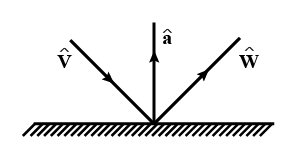
\includegraphics[width=\columnwidth]{20/img.png}
 \caption{}
 \label{fig:img}
 \end{figure}

\end{enumerate}
  
\section*{F  :  Match The Following}
 
 DIRECTIONS (Q. 1-6): Each question contains statements given in two columns, which have to be matched. The statements in Column-I are labelled 1, 2, 3 and 4. while the statements in Columa-II are labelled as a,b,c, d and e. Any given statement in Column-I can have correct matching with ONE OR MORE statement(s) in Column-II. The appropriate bubbles corresponding to the answer to these questions have to be darkened as illustrated in the following example:
If the correct matches are 1-a. s and e: 2-b and c: 3-1 and 2: and 4-d 

\begin{enumerate}
\item Match the following.(2006)\\

\begin{multicols}{2}
column-I \\
column-II

\end{multicols}

\begin{matchtabular}

Two rays $x+y=\mid a\mid$ and $ax-y=1$ intersects eachother in the first quadrant in the interval $a \in (a_0,\infty)$, the value of $a_0$ is &  2 \\
Point $(\alpha,\beta,\gamma)$ lies on the plane $x+y+z=2$.
Let $\vec{a}=\alpha\hat{i}+\beta\hat{j}+\gamma\hat{k}$,$\hat{k} \times \brak{\hat{k}\times\vec{a}}=0$, then $\gamma=$ & $\frac{4}{3}$\\
$\Bigg |\int_{0}^{1}\brak{1-y^2}dy|+\Bigg | \int_{1}^{0}\brak{y^2-1}dy|$ & $\Bigg |\int_{0}^{1}\sqrt{1-x}dx|+\Bigg | \int_{-1}^{0}\sqrt{1-x}dx|$\\
If $\sin A \sin B \sin C+ \cos A\cos B=1$,then the value of $\sin C=$ & 1\\

\end{matchtabular}

\item Consider the following linear equations\\
$ax+by+cz=0$;$bx+cy+az=0$;$cx+ay+bz=0$\\
Match the coditions/expressions in Column I with statements in Column II.(2007)
\begin{multicols}{2}
column-I \\
column-II
\end{multicols}

\begin{matchtabular}
$a+b+c\neq 0$and$a^2+b^2+c^2=ab+bc+ca$ & the equation represent planes meeting only at a single point\\
$a+b+c=0$and$a^2+b^2+c^2 \neq ab+bc+ca$ & the equation represent the line $x=y=z$\\
$a+b+c\neq 0$and$a^2+b^2+c^2 \neq ab+bc+ca$ & the equation representidentical planes.\\
$a+b+c=0$and$a^2+b^2+c^2=ab+bc+ca$ & the equation represent the whole of the three dimensional space.

\end{matchtabular} 

\item Match the statements/expressions given in Column I with the values given in Column II.(2009)

\begin{multicols}{2}
column-I \\
column-II

\end{multicols}

\begin{matchtabular}

Root(s)of the equation $2\sin^2\theta +\sin^22\theta =2$ & $\frac{\pi}{6}$\\
Points of discontinuity of the function $f(x)=\sbrak{\frac{6x}{\pi}\cos\frac{3x}{\pi}}$,f where [y] denotes the largest integer less than or equal to y & $\frac{\pi}{4}$\\
Volume of the parallelopiped with it's edges represented by the vectors $\hat{i}+\hat{j},\hat{i}+2\hat{j}$ and $\hat{i}+\hat{j}+\pi \hat{k}$ & $\frac{\pi}{2}$\\
Angle beteen vector $\vec{a} and \vec{b}$ where $\vec{a}, \vec{b} and \vec{c}$ are unit vectors satisfying $\vec{a}+\vec{b}+\sqrt{3}\vec{c}=0$ & $\pi$

\end{matchtabular}

\item Match the statements/expressions given in Column I with the values given in Column II.(2009)

\begin{multicols}{2}
column-I \\
column-II

\end{multicols}

\begin{matchtabular} 

The number of solution of the given $x e^{\sin x} -\cos x=0$ in the interval $\sbrak{0,\frac{\pi}{2}}$ & 1\\
Value(s) of k for which the planes $kx+4y+z=0,4x+ky+2z=0$ and $2x+2y+z=0$ intersects in a straight line.& 2\\
Value(s) of k for which $\mid x-1 \mid +\mid x-2\mid +\mid x+1\mid+\mid x+2\mid=4k$ has integer solution(s) & 4\\
If $y'=y+1$ and $y(0)=1$,then value(s) of y(1 and 2) & 5\\

\end{matchtabular}

\item Match the statements/expressions given in Column I with the values given in Column II.(2009)

\begin{multicols}{2}
column-I \\
column-II

\end{multicols}

\begin{matchtabular} 

A line from the origin meets the lines $\frac{x-2}{1}=\frac{y-1}{-2}=\frac{z+1}{1}$ and $\frac{x-\frac{8}{3}}{2}=\frac{y+3}{-1}=\frac{z-1}{1}$ at P and Q respectively.If length PQ=d,thej $d^2$ is & -4\\
The value of x satisfying $\tan^{-1}\brak{x+3}-\tan^{-1}\brak{x-3}=\sin^{-1}\sbrak{\frac{3}{5}}$ are & 0\\
Non-zero vectors $\vec{a}, \vec{b}$ and $\vec{c}$ satisfy $\vec{a}\cdot\vec{b}=0$.$\brak{\vec{b}-\vec{a}}\cdot \brak{\vec{b}+\vec{c}}=0$ and $2\mid \vec{b}+\vec{c}\mid=\mid \vec{b}-\vec{a}\mid$. If $\vec{a}=\mu\vec{b}+4\vec{c}$,then the possible values of $\mu$ are & 4\\
Let f be the function on $[-\pi,\pi]$ given by $f(0)=9$ and $f(x)=\frac{\sin\frac{9x}{2}}{\sin\frac{x}{2}} $ for $x\neq 0$. The value of $\frac{2}{\pi}\int_{-\pi}^{\pi}f(x)dx$ is & 5\\    & 6\\


\end{matchtabular}


\item Match the statements/expressions given in Column I with the values given in Column II.(2010)

\begin{multicols}{2}
column-I \\
column-II

\end{multicols}

\begin{matchtabular} 

If $\vec{a}=\hat{j}+\sqrt{3}\hat{k},\vec{b}=-\hat{j}+\sqrt{3}\hat{k}$ and $\vec{c}=\sqrt[2]{3}\hat{k}$ form a triangle, then the internal angle of the triangle between $\vec{a}$ and $\vec{b}$ is & $\frac{\pi}{6}$\\
If $\int_{a}^{b}\brak{f(x)-3x}dx=a^2-b^2$, then the value of $f\sbrak{\frac{\pi}{6}}$ is  & $\frac{2\pi}{3}$\\
The value of $\frac{\pi^2}{ln^3} \int_{\frac{5}{6}}^{\frac{7}{6}}\sec(\pi  x)dx$ is & $\frac{\pi}{3}$\\
The maximum vaalue of $\Bigg | arg\sbrak{\frac{1}{1-z}}\Bigg |  for \mid z \mid =1,z\neq 1$ is given by & $\pi$\\ & $\frac{\pi}{2}$\\


\end{matchtabular}

DIRECTIONS (Q. 7-9): Each question has matching lists have chances (p),(q),(r) and (s) out of which ONLY ONE  is correct.

\item Match List I with  List II and select the answer using the code given below the list

\begin{multicols}{2}
List-I \\
List-II

\end{multicols}

\begin{matchtabular} 
Volume of parallelopiped determined by vectors $\vec{a},\vec{b}$ and $\vec{c}$ is 2.Then the volume of parallelopiped determined by vectors $2\brak{\vec{a}\times\vec{b}},3\brak{\vec{b}\times\vec{c}}$ and $2\brak{\vec{c}\times\vec{a}}$ is  & 100\\
Volume of parallelopiped determined by vectors $\vec{a},\vec{b}$ and $\vec{c}$ is 5.Then the volume of parallelopiped determined by vectors $3\brak{\vec{a}+\vec{b}},3\brak{\vec{b}+\vec{c}}$ and $2\brak{\vec{c}+\vec{a}}$ is  & 30\\
Area of triangle with adjcent sides determined by the vectors  $\vec{a}$ and $\vec{b}$ is 20. Then the area of triangle with adjcent sides determined by the vectors $\brak{3\vec{a}+2\vec{b}}$ and $\brak{\vec{a}-\vec{b}}$ is & 24\\
Area of parallelogram with adjcent sides determined by the vectors  $\vec{a}$ and $\vec{b}$ is 30. Then the area of parallelogram with adjcent sides determined by the vectors $\brak{\vec{a}+\vec{b}}$ and $\vec{a}$ is & 60\\

\end{matchtabular}

Codes:\\
 \begin{tabular}{c c c c c}
             & 1 & 2 & 3 & 4 \\
         (p) & d & b & c & a \\
         (q) & b & c & a & d \\
         (r) & c & d & a & b \\
         (s) & a & d & c & b \\
        \end{tabular}
 
 
\item Consider the lines $L_1: \frac{x-1}{2}=\frac{y}{-1}=\frac{z+3}{1}$,$L_2:\frac{x-4}{1}=\frac{y+3}{1}=\frac{z+3}{2}$ and the planes $P_1: 7xy+2z=3$, $P_2=3x+5y-6z=4$.Let $ax+by+cz=d$ be the equation of the plane pasing through the point of intersection of lines $L_1$ and $L_2$ and erpedicular to plane $P_1$ and $P_2$.\\ (2013)


Match List I with  List II and select the answer using the code given below the list

 
\begin{multicols}{2}
List-I \\
List-II

\end{multicols}

\begin{matchtabular} 
a = & 13\\
b = & -3\\
c = &  1\\
d = & -2\\
 
\end{matchtabular}
 
Codes:\\
\begin{tabular}{c c c c c}
             & 1 & 2 & 3 & 4 \\
         (p) & c & b & d & a \\
         (q) & a & c & d & b \\
         (r) & c & b & a & d \\
         (s) & b & d & a & c \\
 \end{tabular}
\item Match List I with  List II and select the answer using the code given below the list  (2014)
 
\begin{multicols}{2}
List-I  \\
List-II  \\
7
\end{multicols}

\begin{matchtabular} 

Let $y(x)=\cos\brak{2\cos^{-1}x},x\in \sbrak{-1,1},x\neq \pm \frac{\sqrt{3}}{2}$. Then $\frac{1}{y(x)} \bigg\{ \brak{x^2-1}\frac{d^{2}y(x)}{dx^2}+\frac{dy(x)}{dx}\bigg\}$ equals & 1\\
Let $A_1,A_2....A_n(n>2)$ be the vertices of a regular polygon of n sides with it's center at the origin. Let $\vec{a_k}$ be the position vector of the points $A_k,k=1,2,...,n$. If $ \Bigg | \sum_{k=1}^{n-1}\sbrak{\vec{a_k}\times \vec{a_k+1}}\Bigg |$=$\Bigg | \sum_{k=1}^{n-1}\sbrak{\vec{a_k}\cdot \vec{a_k+1}}\Bigg | $,then the minimum value of n is & 2\\
If the normal from the point $p(h,1)$ on the ellipse $\frac{x^2}{6}+\frac{y^2}{3}=1$ is perpendicular to the line $x+y=8$, then the value of h & 8\\
Number of positive solution satisfying the equation $\tan^-1\frac{1}{2x+1}+\tan^-1\frac{1}{4x+1}=\tan^-1\frac{2}{x^2}$ is & 9\\

\end{matchtabular}
Codes:\\
\begin{tabular}{c c c c c}
             & 1 & 2 & 3 & 4 \\
         (p) & d & c & b & a \\
         (q) & b & d & c & a \\
         (r) & d & c & a & b \\
         (s) & b & d & a & c \\
 \end{tabular}

DIRECTIONS (Q.10-11): Refer to directions (1-6).
\item Match the following: (2015)

\begin{multicols}{2}
column-I \\
column-II

\end{multicols}

\begin{matchtabular} 
In $R^2$, if the magnitude of the projection vector of the vector $\alpha \hat{i}+\beta \hat{j}$ on $\sqrt{3}\hat{i}+\hat{j}$ is $\sqrt{3}$ and if $\alpha =2+\sqrt{3}\beta$, the possible value of $\mid \alpha \mid$ is/are & 1\\
Let a and b be real numbers such that the function $f(x)= \bigg \{$
 \begin{tabular}{ c c }
 $-3ax^{2}-2$, & $x < 1$ \\ 
 $ bx+a^2$, & $x\ge 1 $ \\
 \end{tabular} 
is differentiable for all $x \in R$ Then possible value of a is (are) & 2 \\
Let $\mu\neq 1$ be a complex cube root of unity. If $\brak{3-3\mu+2\mu^2}^{4n+3}+\brak{2+3\mu-3\mu^2}^{4n+3}+\brak{-3+2\mu+3\mu^2}^{4n+3}=0$ then possible value(s) of n is (are) & 3\\
Let the harmonic mean of two possitive real numbers a and b be 4. If q is a positive real number such that a,5,q,b is an arithmetic progression, then the value(s) of $\mid q-a \mid$ is (are) & 4 \\ & 5\\


\end{matchtabular}

\item match the following:  (2015)

\begin{multicols}{2}
column-I \\
column-II

\end{multicols}

\begin{matchtabular} 
In a triangle $\triangle XYZ$, let a,b and c be the length of the sides opposite to the angles X,Y and Z respectively. If $2\brak{a^2-b^2}=1$ and  $\lambda=\frac{\sin X-Y}{\sin Z}$, then possible values of n for which $\cos (n\pi\lambda)=0$ is(are) & 1\\
In a triange $\triangle XYZ$, let a,b and c be length of the sides opposite to the angles X,Y and Z respectively. If $1+\cos 2X-2\cos 2Y=2\sin X \sin Y$, then possible value(s) of $\frac{a}{b}$ is (are) &2\\
In $R^2$, let $\sqrt{3}\hat{i}+\hat{j},\hat{i}+\sqrt{3}\hat{j}$ and $\beta\hat{i}+\brak[1-\beta\hat{j}$ be position vectors of X,Y and Z with respect to origin O,respectively . If the distance of Z from the bisector of the acute angle of $\vec{OX}$ with $\vec{OY}$is $\frac{3}{\sqrt{2}}$, then possible value(s) of $\mid \beta \mid $ is (are) & 3\\
Suppose that $F(\alpha)$ denotes the area of the region bounded by $x=0,x=2,y^{2}=4x$ and $y=\mid \alpha x-1 \mid+\mid \alpha x-2 \mid+\alpha x $  where $\alpha \in {0,1}$ . Then the value(s) of $F(\alpha)+\frac{8}{3}\sqrt{2}$, when $\alpha=0$ and $\alpha=1$ is(are) & 5\\ & 6\\

\end{matchtabular}
\end{enumerate}
\section*{F  :  Comprehension Based Questions}

Consider the lines $L_1:\frac{x+1}{3}=\frac{y+2}{1}=\frac{z+1}{2}$ $L_2:\frac{x-2}{1}=\frac{y+2}{2}=\frac{z-3}{3}$

\begin{enumerate}
\item The unit vector perpendicular to both $L_1$ and $L_2$ is  (2008)
\begin{enumerate}
\item $\frac{-\hat{i}+7\hat{j}+7\hat{k}}{\sqrt{99}}$
\item $\frac{-\hat{i}-7\hat{j}+5\hat{k}}{\sqrt[5]{3}}$
\item $\frac{-\hat{i}+7\hat{j}+5\hat{k}}{\sqrt[5]{3}}$
\item $\frac{7\hat{i}-7\hat{j}-\hat{k}}{\sqrt{99}}$
\end{enumerate}
\item The shortest distance between $L_1$ and $L_2$ is  (2008)
\begin{enumerate}
\item $\frac{17}{\sqrt{3}}$ 
\item 0
\item $\frac{41}{\sqrt[5]{3}}$ 
\item $\frac{17}{\sqrt[5]{3}}$ 
\end{enumerate}
\item The distance of the point(1,1,1) from the plane passing through the point(-1,-2,-1) wwhose normal is perpendicular to both the lines $L_1$ and $L_2$ is  (2008)
\begin{enumerate}
\item  $\frac{2}{\sqrt{75}}$
\item  $\frac{7}{\sqrt{75}}$  
\item  $\frac{13}{\sqrt{75}}$ 
\item  $\frac{22}{\sqrt{75}}$ 
\end{enumerate}
\end{enumerate}

\section*{H   :  Assertion And Reason Type Questions}

\begin{enumerate}
\item Consider the plane $3x-6y-2z=15$ and $2x+y-2z=5$.
 STATEMENT-1: The parametric equations of the line of intersection of the given planes are $x=3+14t$,$y=1+2t$ and $z=15t$ because
 STATEMENT-2: The vector $14i + 2j+15k$ is parallel to the line of intersection of given planes. (2007)
\begin{enumerate}
\item Statement-1 is True, Statement-2 is True; Statement-2 is a correct explanation for Statement-1 
\item Statement-1 is True, Statement-2 is True; Statement-2 is NOT a correct explanation for Statement-1
\item Statement-1 is True, Statement-2 is False
\item Statement-1 is False, Statement-2 is True.
\end{enumerate}
\item Let the vectors $\vec{PO}, \vec{OR}, \vec{RS}, \vec{ST}, \vec{TU}$ and $\vec{JP}$ represent the sides ofa regular hexagon.
STATEMENT-1: $\vec{PQ}\times\brak{\vec{RS}+\vec{ST}}\neq \vec{0}$.because
 STATEMENT-2: $\vec{PQ}\times\vec{RS}=\vec{0}$ and $\vec{PQ}\times \vec{ST}\neq \vec{0}$
 (2007)
 \begin{enumerate}
\item Statement-1 is True, statement-2 is True; Statement-2 is a correct explanation for Statement-1.
\item Statement-1 is True, Statement-2 is True, Statement2 is NOT a correct explanation for Statement-1
\item  statement-1 is True, Statement-2 is False
\item  Statement-1 is False, Statement-2 is True.
\end{enumerate}
\item Consider three planes $P_1:x-y+z=1$ $x+y-z=1$ $x-3y+3z=2$ let $L_1,L_2,L_3$ be the lines of intersection of the planes $P_2$ and $P_3$,$P_3$ and $P_1$ , $P_2$ and $P_1$ respectively.\\
STATEMENT-1Z: At least two of the lines $L_1, L_2$ and $L_3$ are non-parallel and\\
STATEMENT-2: The three planes dose not have a common point. (2008)
\begin{enumerate}
\item STATEMENT -1 is True, STATEMENT -2 is True; STATEMENT - 2 is a correct explanation for STATEMENT- 1
\item STATEMENT - 1 is True, STATEMENT - 2 is True; STATEMENT - 2 is NOT a correct explanation for STATEMENT- 1
\item STATEMENT-1 is True, STATEMENT -2 is False
\item STATEMENT - 1 is False, STATEMENT-2 is True
\end{enumerate}

\end{enumerate}

\section*{I    : Integer Value Correct Type }

\begin{enumerate}
\item If $\vec{a}$ and $\vec{b}$ are vectors in space given by $\vec{a}=\frac{\hat{i}-2\hat{j}}{\sqrt{5}}$ and $\vec{b}=\frac{2\hat{i}+\hat{j}+3\hat{k}}{\sqrt{14}}$,then find the value of $\brak{2\vec{a}+2\vec{b}}\cdot\sbrak{\brak{\vec{a}\times\vec{b}}\times\brak{\vec{a}-2\vec{b}}}$.(2010)
\item If the distance between the plane $Ax-2y +z=d$ and the plane containing the lines 
$\frac{x-1}{2}=\frac{y-2}{3}=\frac{z-3}{4}$ and $\frac{x-2}{3}=\frac{y-3}{4}=\frac{z-4}{5}$ is $\sqrt{6}$ then find $\mid d \mid$.(2010)
\item Let $\vec{a}=-\hat{i}-\hat{k},\vec{b}=-\hat{i}+\hat{j}$ and $\vec{c}=\hat{i}+2\hat{j}+3\hat{k}$ be three given vectors. If $\vec{r}$ is a vector such that $\vec{r} \times\vec{b}=\vec{c}\times\vec{b}$ and $\vec{r}\cdot\vec{a}=0$, then the value of $\vec{r}\cdot\vec{b}$ is (2011)
\item If $\vec{a},\vec{b}$ and $\vec{c}$ are unit vectors satisfying $\mid \vec{a}-vec{b}\mid^{2}+\mid \vec{b}-vec{c}\mid^{2}+\mid +\mid \vec{c}-vec{a}\mid^{2}+\mid=9$, then $2\vec{a}+5\vec{b}+5\vec{c}$ is (2012)
\item Consider the set of eight vectors $V={a\hat{i}+b\hat{j}+c\hat{k};a,b,c\in {-1,1} }$. Three non-coplanar vectors can be chosen from V in $2^p$ ways. Then p is (2013)
\item A pack contains n cards numbered from 1 to n. Two consecutive numbered cards are removed from the pack and the sum of the numbers on the remaining cards is 1224. If the
smaller of the numbers on the removed cards is k, then $K-20=$ is (2013)
\item Let $\vec{a},\vec{b}$ and $\vec{c}$ be three non-coplanar unit vectors such that the angle between every pair of them is $\frac{\pi}{3}$. If $\vec{a}\times\vec{b}+\vec{b}\times\vec{c}=\overrightarrow{pa}+\overrightarrow{qb}+\overrightarrow{rc}$, where p,q and r are scalars then the value of $\frac{p^{2}+2q^{2}+r^{2}}{q^2}$is (2014)
\item  Suppose that $\vec{p},\vec{q}$ and $\vec{r}$ are three non-coplanar unit vectors i $R^3$.Let the components of vector $\vec{s}$ along $\vec{p},\vec{q}$ and $\vec{r}$ be 4,3 and 5 respectively. If the components of this vector $\vec{s}$ along $\brak{-\vec{p}+\vec{q}+\vec{r}}$,$\brak{\vec{p}-\vec{q}+\vec{r}}$ and $\brak{-\vec{p}-\vec{q}+\vec{r}}$ are x,y and z respectively, then the value of $2x+y+z$ is (2015)
\item Let $\vec{a}$ and $\vec{b}$ be two unit vectors such that $\vec{a}\cdot\vec{b}=0$. For some $x,y\in R$, let $\vec{c}=x\vec{a}+y\vec{b}+\brak{\vec{a}\times\vec{b}}$. If $\vec{c}=2$ and the vector $\vec{c}$ is inclined at the same angle $\alpha$ to both $\vec{a}$ and $\vec{b}$ then the value of $8\cos^2\alpha$ is .......(2018)
\item Let P be a point in  the first octant, whose image Qin the plane $x+y=3$(that is,the line segment PQ is perpendicular to the plane $x+y=3$ end the mid-point of PQ lies in the planr $x=y=3$)lies on the z-axis.Let the distance of P from the x-axis be 5. If R is the image of P in the xy-plane,then the length of PR is.....(2018)
\item Consider the cube in the first octant with sides OP,OQ and OR of length 1, along the a-axis and z-axis,respectively,where $O(0,0,0)$ is the origin. Let $S\sbrak{\frac{1}{2},\frac{1}{2},\frac{1}{2}}$ be the center of the cube and T be the vertex of the cube opposite to the origin O such that S lies on the diagonal OT. If $\vec{p}=\overrightarrow{SP},\vec{q}=\overrightarrow{SQ},\vec{r}=\overrightarrow{SR}$ and $\vec{t}=\overrightarrow{ST}$, then the value of $\mid \brak{\vec{p}\times\vec{q}}\times\brak{\vec{r}\times\vec{t}}\mid$ is ......(2018)
\item Three lines are given by $\vec{r}=\lambda \hat{i},\lambda \in R$;$\vec{r}=\mu \brak{\hat{i}+\hat{j}},\mu \in R$ and $\vec{r}=\gamma\brak{\hat{i}+\hat{j}+\hat{k},\gamma\in R}$. Let the lines cuts the plane $x+y+z=1$ at the points A,B and C respectively. If the area of the triangle ABC is $\triangle$ then the value of $\brak{6\triangle^2}$ equals ......(2019)
\item Let $\vec{a}=2\hat{i}+\hat{j}-\hat{k}$ and $\vec{b}=\hat{i}+2\hat{j}-\hat{k}$ be two vectors. Consider a vector $\vec{c}=\alpha\vec{a}+\beta\vec{b},\alpha,\beta \in R$. If the projection of $\vec{c}$ on the vector $\brak{\vec{a}-\vec{b}}$ is $\sqrt[3]{2}$, then the minimum vakue of $\sbrak{\vec{c}-\brak{\vec{a}\times\vec{b}}}\vec{c}$ equals.........(2019)

\end{enumerate} 
\section*{Section-B    [JEE Advanced/IIT-JEE]}
\section*{A    :  Fill in the Blanks}

\begin{enumerate}
\item A plane which passes through the point (3, 2, 0) and the line $\frac{x-4}{1}=\frac{y-7}{5}=\frac{z-4}{4}$ is (2002)
\begin{enumerate}
\item $x-y+z=1$
\item $x+y+z=5$
\item $x+2y-z=1$
\item $2x-y+z=5$
\end{enumerate}
\item If  $\mid \vec{a} \mid =4$,$\mid \vec{b}  \mid =2$ and the angle between $\vec{a}$ and $\vec{b}$ is $\frac{\pi}{6}$ then $\brak{\vec{a}\times\vec{b}}^2$ is equal to (2002)
\begin{enumerate}
\item  48
\item 16
\item $\vec{a}$
\item None of these
\end{enumerate}
\item If $\vec{a},\vec{b},\vec{c}$ are vectors such that 
$
\begin{bmatrix}
\vec{a} & \vec{b} & \vec{c} =4
\end{bmatrix}$
then 
$
\begin{bmatrix}
 \vec{a}\times\vec{b} &\vec{b}\times \vec{c} & \vec{c}\times\vec{a}
\end{bmatrix}$=
\begin{enumerate}
\item 16
\item 64 
\item 4 
\item 8
\end{enumerate}
\item If $\vec{a},\vec{b},\vec{c}$ are vectors show that $\vec{a}+\vec{b}+\vec{c}=0$ and 
 $\mid \vec{a} \mid=7,\mid \vec{b} \mid=5,\mid \vec{c} \mid=3 $ then angle between vector $\vec{b}$ and $\vec{c}$ is (2002)
\begin{enumerate}
\item  $60^\circ $
\item  $30^\circ $
\item  $45^\circ $
\item  $90^\circ $
\end{enumerate}
\item If $\mid \vec{a} \mid=5,\mid \vec{b} \mid=4,\mid \vec{c} \mid=3 $ thus what will be the value of $\mid \vec{a} \cdot \vec{b}+\vec{b}\cdot\vec{c}+\vec{c}\cdot\vec{a} \mid$, given that $\vec{a}+\vec{b}+\vec{c}=0$
\begin{enumerate}
\item 25
\item 50
\item -25
\item -50
\end{enumerate}
\item If the vector $\vec{c},\vec{a}=x\hat{i}+y\hat{j}+z\hat{k}$,$\vec{b}=\hat{j}$ are such that $\vec{a},\vec{b},\vec{c}$ form a right handed system then $\vec{c}$ is
\begin{enumerate}
\item $z\hat{i}-x\hat{k}$
\item $\vec{0}$
\item $y\hat{j}$
\item $-z\hat{i}+x\hat{k}$
\end{enumerate}
\item $\vec{a}=3\hat{i}-5\hat{j}$ and $\vec{b}=6\hat{i}+3\hat{j}$ are two vectors and $\vec{c}$ is a vector such that $\vec{c}=\vec{a}\times\vec{b}$ then $\mid \vec{a}\mid:\mid \vec{b} \mid:\mid \vec{c}\mid$(2002)
\begin{enumerate}
\item $\sqrt{34}:\sqrt{45}:\sqrt{39}$
\item $\sqrt{34}:\sqrt{45}:39$
\item 34:39:45
\item 39:35:34
\end{enumerate}
\item IF $\vec{a}\times\vec{b}=\vec{b}\times\vec{c}=\vec{c}\times\vec{a}$ then $\vec{a}+\vec{b}+\vec{c}=$
\begin{enumerate}
\item abc
\item -1
\item 0
\item 2
\end{enumerate}
\item The d.r. of normal to the plane through $(1, 0, 0), (0, 1,0)$ which makes an angle$\frac{\pi}{4}$ with plane $x+y=3$ are (2002)
\begin{enumerate}
\item  1,$\sqrt{2}$,1
\item  1,1,$\sqrt{2}$
\item  1,1,2
\item  $\sqrt{2}$,1,1
\end{enumerate}
\item Let $\vec{u}=\hat{i}+\hat{j}$,$\vec{v}=\hat{i}-\hat{j}$ and $\vec{w}=\hat{i}+2\hat{j}+3\hat{k}$. If $\hat{n}$ is a unit vector such that $\vec{u}\cdot\hat{n}=0$ and  $\vec{v}\cdot\hat{n}=0$ then $\mid \vec{w}\cdot\hat{n}\mid$ is equals to (2003)
\begin{enumerate}
\item 3
\item 0
\item 1
\item 2
\end{enumerate}
\item  A particle acted on by constant forces $4\hat{i}+\hat{j}-3\hat{k}$ and $3\hat{i}+\hat{j}-\hat{k}$ is displaced from the point $\hat{i}+2\hat{j}-3\hat{k}$to the point $5\hat{i}+4\hat{j}+\hat{k}$. The total work done by the force is (2003)
\begin{enumerate}
\item 50 units
\item 20 units
\item 30 units
\item 40 units
\end{enumerate}
\item The vector $\overrightarrow{AB}=3\hat{i}+4\hat{k} \& \overrightarrow{AC}= 5\hat{i}-2\hat{j}+4\hat{k}$ are the sides of triangle ABC. The length of the median through A is (2003)
\begin{enumerate}
\item $\sqrt{288}$
\item $\sqrt{18}$
\item $\sqrt{72}$
\item $\sqrt{33}$
\end{enumerate}
\item The shortest distance from the plane $12x+4y+3z=327$ to the sphere $x^2+y^2+z^2+4x-2y-6z=155$ is
\begin{enumerate}
\item 39
\item 26 
\item $11\frac{4}{13}$
\item 13
\end{enumerate}
\item The two lines $x=ay+b$, $z=cy+d$ and $x=a^{}y+b^{}$, $z=c^{}y+a^{}$ will be perpendicular, if and only if (2003)
\begin{enumerate}
\item $aa^{'}+cc^{'}+1=0$
\item $aa^{'}+bb^{'}+cc^{'}+1=0$
\item $aa^{'}+bb^{'}+cc^{'}=0$
\item $\brak{a+a^{'}}\brak{b+b^{'}}+\brak{c+c^{'}}$
\end{enumerate}
\item The lines $\frac{x-2}{1}=\frac{y-3}{1}=\frac{z-4}{-k}$ and $\frac{x-1}{k}=\frac{y-4}{1}=\frac{z-5}{1}$ are coplanar if (2003)
\begin{enumerate}
\item k=3 or -2
\item k= 0 or -1
\item k= 1 or -1
\item k=0 or -3
\end{enumerate}
\item If $\vec{a},\vec{b} ,\vec{c}$ are three vectors such that $\vec{a}+\vec{b}+\vec{c}=0$,$\mid \vec{a} \mid=1$,$\mid \vec{b} \mid=2$ and $\mid \vec{c} \mid=3$ then $\vec{a}\cdot\vec{b}+\vec{b}\cdot\vec{c}+\vec{c}\cdot\vec{a}$ is equal to (2003)
\begin{enumerate}
\item 1
\item 0
\item -7 
\item 7
\end{enumerate}
\item The radius of the circle in which the sphere $x^2+y^2+z^2+2x-2y-4z-19=0$ is cut by the plane $x+2y+2z+7=0$ (2003)
\begin{enumerate}
\item 4
\item 1
\item 2 
\item 3
\end{enumerate}
\item A tetrahedron has vertices at$O(0,0,0),A(1,2,1)B(2,1,3)$ and $C(-1,1,2)$. Then the angle between the faces OAB and ABC will be (2003)
\begin{enumerate}
\item $90^\circ$ 
\item $\cos^-{1}\frac{19}{35}$ 
\item $\cos^-{1}\frac{17}{31}$ 
\item $30^\circ$ 
\end{enumerate}
\item If $\begin{vmatrix}
 a & a^2  & 1+a^3\\
 b   & b^2 & 1+b^3\\
 c    & c^2 & 1+c^3
\end{vmatrix}=0$ \\ and vectors $(1,a,a^2)$,$(1,b,b^2)$ and $(1,c,c^2)$ are non-coplanar, then the product abc equals (2003)
\begin{enumerate}
\item 0
\item 2
\item -1
\item 1
\end{enumerate}
\item  Consider points A,,B,C and D  with position vectors $7\hat{i}-4\hat{j}+7\hat{k}$,$\hat{i}-6\hat{j}+10\hat{k}$,$-\hat{i}-3\hat{j}+\hat{k}$ and $5\hat{i}-\hat{j}+\hat{k}$ respectively. Then ABCD is a (2003)
\begin{enumerate}
\item parllelogram but not a rhombus
\item square
\item rhombus
\item rectangle
\end{enumerate}
\item If $\vec{u},\vec{v}$ and $\vec{w}$ are three non-planar vectors then $\brak{\vec{u}+\vec{v}-\vec{w}}\cdot\brak{\vec{u}-\vec{w}}\times\brak{\vec{v}-\vec{w}}$ equals (2003)
\begin{enumerate}
\item $3\vec{u}\cdot\vec{v}\times\vec{w}$
\item 0
\item $\vec{u}\cdot\vec{v}\times\vec{w}$
\item $3\vec{u}\cdot\vec{w}\times\vec{v}$
\end{enumerate}
\item Two system of rectangular axes have the same origin. If a plane cuts them at distances a,b,c and $a^{'},b^{'},c^{'}$ from the origin then (2003)
\begin{enumerate}
\item $\frac{1}{a^2}+\frac{1}{b^2}+\frac{1}{c^2}-\frac{1}{a'^2}-\frac{1}{b'^2}-\frac{1}{c'^2}=0$
\item $\frac{1}{a^2}+\frac{1}{b^2}+\frac{1}{c^2}+\frac{1}{a'^2}+\frac{1}{b'^2}+\frac{1}{c'^2}=0$
\item $\frac{1}{a^2}+\frac{1}{b^2}-\frac{1}{c^2}+\frac{1}{a'^2}+\frac{1}{b'^2}-\frac{1}{c'^2}=0$
\item $\frac{1}{a^2}-\frac{1}{b^2}-\frac{1}{c^2}+\frac{1}{a'^2}-\frac{1}{b'^2}-\frac{1}{c'^2}=0$
\end{enumerate}
\item Distance between two parallel planes $2x+y+2z=8$ and $4x+2y+4z+5=0$ is (2004)
\begin{enumerate}
\item $\frac{5}{2}$
\item $\frac{9}{2}$
\item $\frac{7}{2}$
\item $\frac{3}{2}$
\end{enumerate}
\item A line with dircction cosines proportional to 2, 1,2 meets each of the lines each of the lines $x=y+a=z$ and $x+a=2y=2z$. The coordinates of each of the points of intersection is given by (2004)
\begin{enumerate}
\item $(2a,3a,3a),(2a,a,a)$
\item $(3a,2a,2a),(a,a,a)$
\item $(3a,2a,3a),(a,a,2a)$
\item $(3a,3a,3a),(a,a,a)$
\end{enumerate}
\item If the straight lines $x=1+s,y=-3-\lambda s,z=1+\lambda s$ and $x=\frac{t}{2},y=1+t,z=2-t$ with parameters s and t respectively, are co-planar then $\lambda$ is (2004)
\begin{enumerate}
\item 0
\item -1
\item $-\frac{1}{2}$
\item -2
\end{enumerate}
\item The intersection of the spheres $x^2+y^2+z^2+7x-2y-z=13$ and $x^2+y^2+z^2-3x+3y+4z=8$ is the same as the intersection of the sphere and the plane (2004)
\begin{enumerate}
\item $2x-y-z=1$
\item $x-2y-z=1$
\item $x-y-2z=1$
\item $x-y-z=1$
\end{enumerate}
\item Let $\vec{a},\vec{b}$ and $\vec{c}$ are three non-zero coplanar vectors such that no two of these are collinear. I the vector $\vec{a}+2\vec{b}$ is collinear with $\vec{c},\vec{b}+3\vec{c}$ is collinear with $\vec{a}$($\lambda$ being some non-zero scalar then $\vec{a}+2\vec{b}+6\vec{c}$ is equals (2004)
\begin{enumerate}
\item 0
\item $\lambda \vec{a}$
\item $\lambda \vec{b}$
\item $\lambda \vec{c}$
\end{enumerate} 
\item A particles is acted upon by constant force $4\hat{i}+\hat{j}-3\hat{k}$ and $3\hat{i}+\hat{j}-\hat{k}$ which displace it from a point $\hat{i}+2\hat{j}+3\hat{k}$ to the point $5\hat{i}+4\hat{j}+\hat{k}$.The work done in standard units by the forces is given by (2004)
\begin{enumerate}
\item 15
\item 30
\item 25 
\item 40
\end{enumerate} 
\item If $\vec{a},\vec{b},\vec{c}$ are non coplanar vectors and $\lambda$ is a real number then the vectors $\vec{a}+2\vec{b}+3\vec{c}$ $\lambda\vec{b}+4\vec{c}$ and $\brak{2\lambda-1}\vec{c}$ are non-coplanar for(2004) 
\begin{enumerate}
\item  No value for $\lambda$
\item  All expect one value for $\lambda$
\item  All expect two value for $\lambda$
\item  ALL values of $\lambda$
\end{enumerate}

\item Let $\vec{u},\vec{v},\vec{w}$ be such that $\mid \vec{u} \mid =1, \mid \vec{v}\mid =2$ and $\mid \vec{w} \mid =3$. If the projection $\vec{v}$ along $\vec{u}$ is equal to that of $\vec{w}$ along $\vec{u}$ and $\vec{v}$, $\vec{w}$ are perpendicular to each other then $\vec{u}-\vec{v}+\vec{w}$ equals(2004)
\begin{enumerate}
\item 14
\item $\sqrt{7}$
\item $\sqrt{14}$If the pane 
\item 2
\end{enumerate} 
\item Let $\vec{a},\vec{b},\vec{c}$ are non-zero vectors such that $\brak{\vec{a}\times\vec{b}}\times\vec{c}=\frac{1}{3} \mid \vec{b} \mid  \mid \vec{c} \mid$ $\vec{a}$. If $\theta$ is the acute angle between vectors $\vec{b}$ and $\vec{c}$ then $\sin \theta$ equals (2004)
\begin{enumerate}
\item $\frac{\sqrt[2]{2}}{3}$
\item $\frac{\sqrt{2}}{3}$
\item $\frac{2}{3}$
\item $\frac{1}{3}$
\end{enumerate}
\item If C is the mid-point of AB and P is any point outside AB, then (2005)
\begin{enumerate}
\item $\overrightarrow{PA}+\overrightarrow{PB}=2\overrightarrow{PC}$
\item $\overrightarrow{PA}+\overrightarrow{PB}=\overrightarrow{PC}$
\item $\overrightarrow{PA}+\overrightarrow{PB}+2\overrightarrow{PC}=0$
\item $\overrightarrow{PA}+\overrightarrow{PB}+\overrightarrow{PC}=0$
\end{enumerate}
\item If the angle $\theta$ between the lines $\frac{x+1}{2}=\frac{y-1}{2}=\frac{z-2}{2}$ and the plane $2x-y+\sqrt{\lambda}z+4=0$ is such that $\sin\theta=\frac{1}{3}$ then the value of $\lambda$ is (2005)
\begin{enumerate}
\item  $\frac{5}{3}$
\item $\frac{-3}{5}$
\item $\frac{3}{4}$
\item $\frac{-4}{3}$
\end{enumerate}
\item The angle between the lines $2x=3y=-z$ and $6x=-y=-4z$ is (2005)
\begin{enumerate}
\item $0^\circ$
\item $90^\circ$
\item $45^\circ$
\item $30^\circ$
\end{enumerate}
\item If the plane $2ax-3ay+4az+6=0$ passes through the mid-point of line joining the center of the spheres $x^2+y^2+z^2+6x-8y-2z=13$ and $x^2+y^2+z^2-10x+4y-2z=8$ then a equals (2005)
\begin{enumerate}
\item -1
\item 1
\item -2 
\item 2
\end{enumerate}
\item The distance between the line $\vec{r}=2\hat{i}-2\hat{j}+3\hat{k}+\lambda\brak{\hat{i}-\hat{j}+4\hat{k}}$ and the plane $\vec{r}\cdot\brak{\hat{i}+5\hat{j}+\hat{k}}=5$(2005)
\begin{enumerate}
\item $\frac{10}{9}$
\item $\frac{10}{\sqrt[3]{3}}$
\item $\frac{3}{10}$
\item $\frac{10}{3}$
\end{enumerate}
\item For any vector $\vec{a}$ , the value of $\brak{\vec{a}\times\hat{i}^2}+\brak{\vec{a}\times\hat{j}^2}+\brak{\vec{a}\times\hat{k}^2}$ is equal to (2005)
\begin{enumerate}
\item $3a^-2$
\item $a^-2$
\item $2a^-2$
\item $4a^-2$
\end{enumerate}
\item If non-zero numbers a, b, c are in H.P., then the straight line. $\frac{x}{a}+\frac{y}{b}+\frac{1}{c}=0$ always passes through a fixed point. That point is (2005)
\begin{enumerate}
\item $(-1,2)$
\item $(-1,-2)$
\item $(-1,-2)$
\item $(1,-\frac{1}{2})$
\end{enumerate}
\item Let a, b and c be distinct non-negative numbers. If the vectors $a\hat{i}+a\hat{j}+c\hat{k},\hat{i}+\hat{k},c\hat{i}+c\hat{j}+b\hat{k}$ lie in a plane, then c is (2005)
\begin{enumerate}
\item the Geometric Mean of a and b
\item the Arithmetic Mean of a and b
\item equal to zero
\item  the Harmonic Mean of a and b
\end{enumerate}
\item  If $\vec{a},\vec{b},\vec{c}$ are non-coplanar vectors and $\lambda$ is real number then 
$
\begin{bmatrix}
\lambda\brak{\vec{a}+\vec{b}} & \lambda^2\vec{b} & \lambda\vec{c} =
\end{bmatrix}$
$\begin{bmatrix}
\vec{a} & \vec{b}+\vec{c} & \vec{b} 

\end{bmatrix}
$ for (2005)
\begin{enumerate}
\item exactly one value of $\lambda$
\item no value $\lambda$
\item exactly three value of $\lambda$
\item exactly two value of $\lambda$
\end{enumerate}
\item Let $\vec{a}=\hat{i}-\hat{k},\vec{b}=x\hat{i}+\hat{j}+\brak{1-x}\hat{k}$ and $\vec{c}=y\hat{i}+x\hat{j}+\brak{1+x-y}\hat{k}$. Then $\sbrak{\vec{a},\vec{b},\vec{c}}$ depends on (2005)
\begin{enumerate}
\item only y
\item only x
\item both x and y
\item neither x nor y
\end{enumerate}
\item The plane $x+2y-z=4$ cuts the sphere $x^2+y^2+z^2-x+z-2=0$ in a circle of radius (2005)
\begin{enumerate}
\item 3 
\item 1
\item 2
\item $\sqrt{2}$
\end{enumerate}
\item If $\brak{\vec{a}\times\vec{b}}\times\vec{c}=\vec{a}\times\brak{\vec{b}\times\vec{c}}$ where $\vec{a},\vec{b},\vec{c}$ are any three vectors such that $\vec{a}\cdot \vec{b}\neq =$,$\vec{b}\cdot \vec{c}\neq =$ then $\vec{a}$ and $\vec{c}$ are (2005)
\begin{enumerate}
\item inclined at an angle of $\frac{\pi}{3}$ between them 
\item inclined at an angle of $\frac{\pi}{6}$ between them 
\item perpendicular
\item parallel
\end{enumerate}
\item The values of a, for which points A, B, C with position vectors  $2\hat{i}-\hat{j}+\hat{k},\hat{i}-3\hat{j}-5\hat{k}$ and $a\hat{i}-3\hat{j}+\hat{k}$ respectively are the vertices of a rightangled triangle with $c=\frac{\pi}{2}$ are (2005)
\begin{enumerate}
\item 2 and 1
\item -2 and -1
\item -2 and 1
\item 2 and -1
\end{enumerate}
\item  The two lines $x=ay+b$,$z=cy+d$ and $x=a'y+b',z=c'y+d'$ are perpendicular to each other if (2006)
\begin{enumerate}
\item $aa'+cc'=-1$
\item $aa'+cc'=1$
\item $\frac{a}{a'}+\frac{c}{c'}=-1$
\item $\frac{a}{a'}+\frac{c}{c'}=1$
\end{enumerate}
\item  The image of the point (-1, 3,4) in the plane $x-2y=1$ is (2006)
\begin{enumerate}
\item $\brak{\frac{-17}{3},\frac{-19}{3},4}$
\item (15,11,4)
\item $\brak{\frac{-17}{3},\frac{-19}{3},1}$
\item None of these
\end{enumerate}
\item If a line makes an angle of $\frac{\pi}{4}$ with the positive directions of each of x- axis and y- axis, then the angle that the line makes with the positive direction of the z-axis is (2006)
\begin{enumerate}
\item $\frac{\pi}{4}$
\item $\frac{\pi}{2}$
\item $\frac{\pi}{6}$
\item $\frac{\pi}{3}$
\end{enumerate}
\item If $\vec{u}$ and $\vec{v}$ are unit vectors and $\theta$ is the acute angle between them, then $2\vec{u}\times 3\vec{v}$ is a unit vector for (2007)
\begin{enumerate}
\item no value of $\theta$
\item exactly one value of $\theta$
\item exactly two value of $\theta$
\item more than two values of $\theta$
\end{enumerate}
\item If (2.3, 5) is one end of a diameter of the sphere $x^2+y^2+z^2-6x-12y-2z+20=0$ then the cooordinates of the other end of the diameter are  (2007)
\begin{enumerate}
\item (4,3,5)
\item (4,3,-3)
\item (4,9,-3)
\item (4,-3,3)
\end{enumerate}
\item Let $\vec{a}=\hat{i}+\hat{j}+\hat{k},\vec{b}=\hat{i}-\hat{j}+2\hat{k},\vec{c}=x\hat{i}+(x-2)\hat{j}-\hat{k}$. If the vectors lies in the plane of $\vec{a}$ and $\vec{b}$ , then x equals (2007)
\begin{enumerate}
\item -4
\item -2
\item 0
\item 1
\end{enumerate}
\item Let L be the line of intersection of the planes $2x+3y+z=1$ and $x+3y+2z=2$. If L makes an angle $\alpha$ with the positive x-axis, then $\cos \alpha$ equals (2007)
\begin{enumerate}
\item 1
\item $\frac{1}{\sqrt{2}}$
\item $\frac{1}{\sqrt{3}}$
\item $\frac{1}{2}$
\end{enumerate}
\item The vector $\vec{a}=\alpha\hat{i}+2\hat{j}+\beta\hat{k}$ lies in the plane of the vectors $\vec{b}=\hat{i}+\hat{j}$ and $\vec{c}=\hat{j}+\hat{k}$ and bisects the angle between $\vec{b}$ and $\vec{c}$. Then which one of the following gives possible
values of $\alpha$ and $\beta$ ? (2008) 
\begin{enumerate}
\item $\alpha=2,\beta=2$ 
\item $\alpha=1,\beta=2$ 
\item $\alpha=2,\beta=1$ 
\item $\alpha=1,\beta=1$ 
\end{enumerate}
\item The non-zero Vectors are $\vec{a},\vec{b}$ and $\vec{c}$ are related by $\vec{a}=8\vec{b}$ and $\vec{c}=-7\vec{b}$. Then the angle between $\vec{a}$ and $\vec{c}$ is (2008)
\begin{enumerate}
\item 0
\item $\frac{\pi}{4}$
\item $\frac{\pi}{2}$
\item $\pi$ 
\end{enumerate}
\item The line passing through the points (5, 1, a) and (3, b, 1) crosses the yz-plane at the point $\sbrak{0,\frac{17}{2},\frac{-13}{2}}$. Then (2008)
\begin{enumerate}
\item a=2,b=8
\item a=4,b=6
\item a=6,b=4
\item a=8,b=2
\end{enumerate}
\item If the straight lines $\frac{x-1}{k}=\frac{y-2}{2}=\frac{z-3}{3}$ and $\frac{x-2}{3}=\frac{y-3}{k}=\frac{z-1}{2}$ intersect at a point, then the integer k is equal to (2008)
\begin{enumerate}
\item -5
\item 5
\item 2
\item -2
\end{enumerate}
\item Let the line $\frac{x-2}{3}=\frac{y-2}{-5}=\frac{z+2}{2}$ lie in the plane $x+3y-\alpha z+\beta=0$ then $(\alpha,\beta)$ equals (2009)
\begin{enumerate}
\item (-6,7)
\item (5,-15)
\item (-5,5)
\item (6,-17)
\end{enumerate}
\item The projections of a vector on the three coordinate axis are 6,-3, 2 respectively. The direction cosines of the vector are:(2009)
\begin{enumerate}
\item $\frac{6}{5},\frac{-3}{5},\frac{2}{5}$ 
\item $\frac{6}{7},\frac{-3}{7},\frac{2}{7}$ 
\item $\frac{-6}{7},\frac{-3}{7},\frac{2}{7}$ 
\item -6,-3,2 
\end{enumerate}
\item If $\vec{u},\vec{v},\vec{w}$ are non-coplanar vectors and p, q are real numbers,then the equality 
$
\begin{bmatrix}
3\vec{u} & p\vec{v} & p\vec{w} 
\end{bmatrix}$-
$
\begin{bmatrix}
p\vec{v} &w\vec{v} & q\vec{u}
\end{bmatrix}$-
$
\begin{bmatrix}
2\vec{w} & q\vec{u} & q\vec{v}
\end{bmatrix}$=0 holds for (2009)
\begin{enumerate}
\item exactly two values of (p,q)
\item more than two but, not all values of (p,q)
\item all values of (p,q)
\item exactly one values of (p,q)
\end{enumerate}
\item Let $\vec{a}=\hat{j}-\hat{k}$ and $\vec{c}=\hat{i}-\hat{j}-\hat{k}$. Then the vector $\vec{b}$ satisfying $\vec{a}\times\vec{b}+\vec{c}=0$  and $\vec{a}\cdot\vec{c}=3$  (2010)
\begin{enumerate}
\item  $2\hat{i}-\hat{j}+2\hat{k}$
\item  $\hat{i}-\hat{j}-2\hat{k}$
\item  $\hat{i}+\hat{j}-2\hat{k}$
\item  $-\hat{i}+\hat{j}-2\hat{k}$
\end{enumerate}
\item If the vectors $\vec{a}=\hat{i}-\hat{j}+2\hat{k}$,$\vec{b}=2\hat{i}+4\hat{j}+\hat{k}$ and $\vec{c}=\lambda\hat{i}+\hat{j}+\mu \hat{k}$ are mutualy orthogonal, then $\brak{\lambda,\mu}$ =(2010)
\begin{enumerate}
\item (2,-3)
\item (-2,3)
\item (3,-2)
\item (-3,2)
\end{enumerate}
\item Statement-1:The point A(3, 1, 6) is the mirror image of the point B(1, 3, 4) in the plane $x-y +z=5$ . (2010)
\begin{enumerate}
\item Statement -1 is true, Statement-2 is true; Statement-2 is not a correct explanation for Statement-1
\item Statement-1 is true, Statement-2 is false.
\item Statement -1 is false, Statement-2 is true.
\item Statement - 1 is true, Statement 2 is true; Statement-2 is a correct explanation for Statement-1.
\end{enumerate}
\item A line AB in three-dimensional space makes angles $45^\circ$ and $120^\circ$ with the positive x-axis and the positive y-axis respectively. If AB makes an acute angle $\theta$ with the positive Z-axis, then $\theta$ equals (2010)
\begin{enumerate}
\item $45^\circ$
\item $60^\circ$
\item $75^\circ$
\item $30^\circ$
\end{enumerate}
\item Ifthe angle between the line  $x=\frac{y-1}{2}=\frac{z-3}{\lambda}$ and the plane 
$x+2y+z=4$ is $\cos^-1\sqrt[5]{14}$, then $\lambda$ equals (2011)
\begin{enumerate}
\item $\frac{3}{2}$
\item $\frac{2}{5}$
\item $\frac{5}{3}$
\item $\frac{2}{3}$
\end{enumerate}
\item If $\vec{a}=\frac{1}{\sqrt{10}}\brak{3\hat{i}+\hat{k}}$ and $\vec{b}=\frac{1}{7}\brak{2\hat{i}+3\hat{j}-6\hat{k}}$, then the value of $\brak{2\vec{a}-\vec{b}}\sbrak{\brak{\vec{a}\times\vec{b}}\times\brak{\vec{a}+2\vec{b}}}$ is (2011)
\begin{enumerate}
\item  -3
\item 5
\item 3 
\item -5
\end{enumerate}
\item The vectors $\vec{a}$ and $\vec{b}$ are not perpendicular and  $\vec{c}$  and $\vec{d}$ are two vectors satisfying $\vec{b}\times\vec{c}=\vec{b}\times\vec{d}$ and $\vec{a}\cdot\vec{d}=0$. Then the vector $\vec{d}$ is equal to (2011)
\begin{enumerate}
\item $\vec{c}+\sbrak{\frac{\vec{a}\cdot\vec{c}}{\vec{a}\cdot\vec{b}}}\vec{b}$ 
\item $\vec{b}+\sbrak{\frac{\vec{b}\cdot\vec{c}}{\vec{a}\cdot\vec{b}}}\vec{c}$
\item $\vec{c}-\sbrak{\frac{\vec{a}\cdot\vec{c}}{\vec{a}\cdot\vec{b}}}\vec{b}$
\item $\vec{b}-\sbrak{\frac{\vec{b}\cdot\vec{c}}{\vec{a}\cdot\vec{b}}}\vec{c}$
\end{enumerate}
\item Statement-1: The point A(1,0, 7)) is the mirror image of the point B(1, 6, 3) in the line : $\frac{x}{2}=\frac{y-1}{2}=\frac{z-2}{3}$  \\
Statement-2: The line $\frac{x}{2}=\frac{y-1}{2}=\frac{z-2}{3}$ bisects the line segment joining A(1, 0,7) and B(1, 6, 3). (2011)
\begin{enumerate}
\item Statement-1 is true, Statement-2 is true; Statement-2 is not a correct explanation for Statement-1.
\item Statement-1 is true, Statement-2 is false.
\item Statement-1 is false, Statement-2 is true.
\item Statement-1 is true, Statement-2 is true; Statement-2 is a correct explanation for Statement-1.
\end{enumerate}
\item Let $\vec{a}$ and $\vec{b}$ be two unit vectors. If the vectors $\vec{c}=\hat{a}+2\hat{b}$ and $\vec{d}=5\hat{a}-4\hat{b}$  are perpendicular to each other, then the angle between $\hat{a}$ and $\hat{b}$ is: (2012)
\begin{enumerate}
\item  $\frac{\pi}{6}$ 
\item  $\frac{\pi}{2}$ 
\item  $\frac{\pi}{3}$ 
\item  $\frac{\pi}{4}$ 
\end{enumerate}
\item A equation of a plane parallel to the plane $x-2y+2z-5=0$ and at a unit distance from the origin is: (2012)
\begin{enumerate}
\item  $x-2y+2z-3=0$
\item  $x-2y+2z+1=0$
\item  $x-2y+2z-1=0$
\item  $x-2y+2z+5=0$
\end{enumerate}
\item If the line $\frac{x-1}{2}=\frac{y+1}{3}=\frac{z-1}{4}$ and $\frac{x-3}{1}=\frac{y-k}{2}=\frac{z}{1}$ intersect, then k is equal to: (2012)
\begin{enumerate}
\item -1
\item $\frac{2}{9}$
\item $\frac{9}{2}$
\item 0
\end{enumerate}
\item Let ABCD be a parallelogram such that $\overrightarrow{AB}=q$ and $\overrightarrow{AD}=p$and $\angle BAD$ an acute angle. If $\vec{r}$ is the vector that coincides with the altitude directed from the vertex B to the side AD, then $\vec{r}$ is given by : (2012)
\begin{enumerate}
\item  $\vec{r}=3\vec{q}-\frac{3\brak{\vec{q}\cdot\vec{p}}}{\brak{\vec{p}\cdot\vec{p}}}\vec{p}$
\item  $\vec{r}=-\vec{q}+\frac{3\brak{\vec{q}\cdot\vec{p}}}{\brak{\vec{p}\cdot\vec{p}}}\vec{p}$
\item  $\vec{r}=\vec{q}-\frac{3\brak{\vec{q}\cdot\vec{p}}}{\brak{\vec{p}\cdot\vec{p}}}\vec{p}$
\item  $\vec{r}=-3\vec{q}-\frac{3\brak{\vec{q}\cdot\vec{p}}}{\brak{\vec{p}\cdot\vec{p}}}\vec{p}$
\end{enumerate}
\item Distance between two parallel planes $2x+y+2z=8$ and $4x+2y+4z+5=0$ is (2013)
\begin{enumerate}
\item $\frac{3}{2}$
\item $\frac{5}{2}$
\item $\frac{7}{2}$
\item $\frac{9}{2}$
\end{enumerate}
\item f the line $\frac{x-2}{1}=\frac{y-3}{1}=\frac{z-4}{-k}$ and $\frac{x-1}{k}=\frac{y-4}{2}=\frac{z-5}{1}$ are coplanar, then k can have (2013)
\begin{enumerate}
\item any value 
\item exactly one value
\item exactly two values
\item exactly three values
\end{enumerate}
\item If the vectors $\overrightarrow{AB}=3\hat{i}+4\hat{k}$ and $\overrightarrow{AC}=5\hat{i}-2\hat{j}+4\hat{k}$ are the sides of a triangle ABC, then the length of the median through A is 2013)
\begin{enumerate}
\item $\sqrt{18}$
\item $\sqrt{72}$
\item $\sqrt{33}$
\item $\sqrt{45}$
\end{enumerate}
\item The image of the line  $\frac{x-1}{3}=\frac{y-3}{1}=\frac{z-4}{-5}$ in the plane $2x-y+z+3=0$ is the line : (2014)
\begin{enumerate}
\item $\frac{x-3}{3}=\frac{y+5}{1}=\frac{z-2}{-5}$
\item $\frac{x-3}{-3}=\frac{y+5}{-1}=\frac{z-2}{5}$
\item $\frac{x+3}{3}=\frac{y-5}{1}=\frac{z-2}{-5}$
\item $\frac{x+3}{-3}=\frac{y-5}{-1}=\frac{z+2}{5}$
\end{enumerate}
\item The angle between the lines whose direction cosines satisfy the equation $l+m+n=0$ and $\l^2=m^2+n^2$ is (2014)
\begin{enumerate}
\item $\frac{\pi}{6}$
\item $\frac{\pi}{2}$
\item $\frac{\pi}{3}$
\item $\frac{\pi}{4}$
\end{enumerate}
\item If 
$
\begin{bmatrix}
 \vec{a}\times\vec{b} &\vec{b}\times \vec{c} & \vec{c}\times\vec{a}
\end{bmatrix}$
=$\lambda$
$
\begin{bmatrix}
\vec{a} & \vec{b} & \vec{c}
\end{bmatrix}
$
then $\lambda$ is equal to (2014)
\begin{enumerate}
\item 0
\item 1
\item 2
\item 3 
\end{enumerate}
\item Let $\vec{a},\vec{b}$ and $\vec{c}$ be three non-zero vectors such that no two ofthem are collinear and $\brak{\vec{a}\times\vec{b}}\times \vec{c}=\frac{1}{3}\mid \vec{b} \mid \mid \vec{c} \mid \vec{a}$.If $\theta$ is angle between vectors $\vec{b}$ and $\vec{c}$ , then a value of$\sin \theta$ is: (2015)
\begin{enumerate}
\item $\frac{2}{3}$
\item $\frac{-\sqrt[2]{3}}{3}$
\item $\frac{\sqrt[2]{2}}{3}$
\item $\frac{-\sqrt{2}}{3}$
\end{enumerate}
\item The equation of the plane containing the line $2x-y+z=3$ and $x+y+4z=5$, and parallel to the plane,$x+3y+6z=1$ is :(2015)
\begin{enumerate}
\item $x+3y+6z=7$
\item $2x+6y+12z=-13$
\item $2x+6y+12z=13$
\item $x+3y+6z=-7$
\end{enumerate}
\item  The distance of the point (1, 0, 2) from the point of intesection of the lines $\frac{x-2}{3}=\frac{y+1}{4}=\frac{z-2}{12}$ and the plane $x-y+x=16$ is :(2015)
\begin{enumerate}
\item $\sqrt[3]{21}$
\item 13
\item $\sqrt[2]{14}$
\item 8
\end{enumerate}
\item If the line $\frac{x-3}{2}=\frac{y+2}{-1}=\frac{z-4}{3}$ lies in the plane $lx+my-z=9$ then $l^2+m^2$ is equal to (2016)
\begin{enumerate}
\item 5
\item 2
\item 12
\item 18
\end{enumerate}
\item  Let $\vec{a},\vec{b}$ and $\vec{c}$ be three unit vectors such that $\vec{a}\times\sbrak{\vec{b}\times}\vec{c}=\frac{\sqrt{3}}{2}\sbrak{\vec{b}+\vec{c}}$. If $\vec{b}$ is not parallel to $\vec{c}$ then the angle between $\vec{a}$ and $\vec{c}$ is (2016)
\begin{enumerate}
\item $\frac{2\pi}{3}$
\item $\frac{5\pi}{6}$
\item $\frac{3\pi}{4}$
\item $\frac{\pi}{2}$
\end{enumerate}
\item The distance of the point (1, -5, 9) from the plane $x-y+z=5$ measured along the line $x =y=z$ is: (2016)
\begin{enumerate}
\item  $\frac{10}{\sqrt{3}}$
\item $\frac{20}{3}$
\item $\sqrt[3]{10}$
\item $\sqrt[10]{3}$
\end{enumerate}
\item  Let $\vec{a}=2\hat{i}+\hat{j}-2\hat{k}$ and $\vec{b}=\hat{i}+\hat{j}$ and $\vec{c}$ be a vectors such that $\mid \vec{c}-\vec{a} \mid =3$,$\mid \sbrak{\vec{a}\times\vec{b}}\times \vec{c}\mid=3$ and the angle between $\vec{c}$ and $\vec{a}\times\vec{b}$ is $30^\circ$. Then $\vec{a}\cdot\vec{c}$ is equal to :(2017)
\begin{enumerate}
\item $\frac{1}{8}$
\item $\frac{25}{8}$
\item 2
\item 5
\end{enumerate}
\item  If the image of the point P(1, -2, 3) in the plane,$2x+3y-4z+22=0$  measured parallel to line,$\frac{x}{1}=\frac{y}{4}=\frac{z}{5}$ is Q, then PQ is equal to:(2017)
\begin{enumerate}
\item  $\sqrt[6]{5}$
\item  $\sqrt[3]{5}$
\item  $\sqrt[2]{42}$
\item  $\sqrt{42}$
\end{enumerate}
\item The distance of the point (1, 3, -7) from the plane passing through the point (1, -1, -1), having normal perpendicular to both the lines $\frac{x-1}{1}=\frac{y+2}{-2}=\frac{z-4}{3}$ and $\frac{x-2}{2}=\frac{y+1}{-1}=\frac{z+7}{-1}$ is :(2017)
\begin{enumerate}
\item $\frac{10}{\sqrt{74}}$
\item $\frac{20}{\sqrt{74}}$
\item $\frac{10}{\sqrt{83}}$
\item $\frac{5}{\sqrt{83}}$
\end{enumerate}
\item let $\vec{u}$ be a vector coplanar with the vectors $\vec{a}=2\hat{i}+3\hat{j}-\hat{k}$ and $\vec{b}=\hat{j}+\hat{k}$. If $\vec{u}$ is perpendicular to $\vec{a}$ and $\vec{u}\cdot\vec{b}=24$ , then $\mid \vec{u}\mid^2$ is equal to: (2018)
\begin{enumerate}
\item 315
\item 250
\item 84
\item 336
\end{enumerate}
\item The length of the projection  of the line segment joining the points (5, 1, 4) and (4, 1,3)on the plane,$x+y+z=7$ in: (2018)
\begin{enumerate}
\item $\frac{2}{3}$
\item $\frac{1}{3}$
\item $\sqrt{\frac{2}{3}}$
\item $\frac{2}{\sqrt{3}}$
\end{enumerate}
\item If $\L_1$ is the line of intersetion of the planes $2x-2y+3z-2=0$ and $x-y+z+1=0$ and $L_2$ is the line of intersection of the planes $x+2y-z-3=0$,$3x-y+2z=0$, then the distance of the origin from the plane,containing the lines $\L_1$  and $L_2$ is : (2018)
\begin{enumerate}
\item $\frac{1}{\sqrt[3]{2}}$
\item $\frac{1}{\sqrt[2]{2}}$
\item $\frac{1}{\sqrt{2}}$
\item $\frac{1}{\sqrt[4]{2}}$
\end{enumerate}
\item Let $\vec{a}=\hat{i}-\hat{j}$,$\vec{b}=\hat{i}+\hat{j}+\hat{k}$ and $\vec{c}$ be a vector such that $\vec{a}\times\vec{c}+\vec{b}=\vec{0}$ and $\vec{a}\cdot\vec{c}=4$, then $\mid \vec{c}\mid ^2$ is equal to :(2018)
\begin{enumerate}
\item $\frac{19}{2}$
\item 9
\item 8 
\item $\frac{17}{2}$
\end{enumerate}
\item  The equation of the line passing through (-4,3, 1), parallel to the plane $x+2y-z-5-0$ and intersecting the line $\frac{x+1}{-3}=\frac{y-3}{2}=\frac{z-2}{-1}$ is:(2018)
\begin{enumerate}
\item $\frac{x-4}{2}=\frac{y+3}{1}=\frac{z+1}{4}$
\item $\frac{x+4}{1}=\frac{y-3}{1}=\frac{z-1}{3}$
\item $\frac{x+4}{3}=\frac{y+3}{1}=\frac{z-1}{1}$
\item $\frac{x+4}{-1}=\frac{y-3}{1}=\frac{z-1}{1}$
\end{enumerate}
\item  The plane through the intersection of the planes $x+y+z-1$ and $2x+3y-z+4=0$ and parallel to y-axis also  passes through the point: (2019)
\begin{enumerate}
\item (-3,0,-1)
\item (-3,1,-1)
\item (3,3,-1)
\item (3,2,-1)
\end{enumerate}
\item If the line $\frac{x-1}{2}=\frac{y+1}{3}=\frac{z-2}{4}$ meets the plane,$x+2y+3z=15$ at a point P, then the distance of P from the origin is: (2019)
\begin{enumerate}
\item  $\frac{\sqrt{5}}{2}$
\item $\sqrt[2]{5}$
\item $\frac{9}{2}$
\item $\frac{7}{2}$
\end{enumerate}
\item A plane passing through the points (0, -1,0) and (9, 0, 1) and making an angle $\frac{\pi}{2}$ with the plane $y-z+5=0$, also passes through the point: (2019)
\begin{enumerate}
\item (-$\sqrt{2}$,1,-4)
\item ($\sqrt{2}$,-1,4)
\item (-$\sqrt{2}$,-1,-4)
\item ($\sqrt{2}$,1,4)
\end{enumerate}
\item Let $\vec{\alpha}=3\hat{i}+\hat{j}$ and $\vec{\beta}=2\hat{i}-\hat{j}+3\hat{k}$. If $\vec{\beta}=\vec{\beta_1}-\vec{\beta_2}$, where $\vec{\beta}_1$ is parallel to $\vec{\alpha}$ and $\vec{\beta}_2$ is perpendicular to $\vec{\alpha}$, then $\vec{\beta}_1\times\vec{\beta}_2$ is equal to :(2019)
\begin{enumerate}
\item  $-3\hat{i}+9\hat{j}+5\hat{k}$
\item  $3\hat{i}-9\hat{j}-5\hat{k}$
\item  $\frac{1}{2}\brak{-3\hat{i}+9\hat{j}+5\hat{k}}$
\item  $\frac{1}{2}\brak{3\hat{i}-9\hat{j}-5\hat{k}}$
\end{enumerate}

\end{enumerate}
